% =====================================================================
%  AWG / DDS Function Generator — Engineering Process Report
%  Compile: pdflatex (x2, for cross-references and the ToC)
%  Requires: tcolorbox, cleveref, tikz — all standard in TeX Live full
% =====================================================================
\documentclass[11pt,a4paper]{article}

\usepackage[utf8]{inputenc}
\usepackage[T1]{fontenc}
\usepackage{lmodern}
\usepackage{textcomp}
\usepackage[margin=2.4cm]{geometry}
\usepackage{graphicx}
\usepackage{xcolor}
\usepackage{booktabs}
\usepackage{longtable}
\usepackage{array}
\usepackage{tabularx}
\usepackage{colortbl}
\usepackage{microtype}
\usepackage{pdflscape}
\usepackage{enumitem}
\usepackage{titlesec}
\usepackage{fancyhdr}
\usepackage{parskip}
\usepackage{float}
\usepackage{caption}
\usepackage{tikz}
\usepackage[most]{tcolorbox}

% ------------------------------------------------------------ colours
\definecolor{accent}{HTML}{2E4B3F}      % deep green — headings, links
\definecolor{accentline}{HTML}{9DB3A8}  % muted green — rules, ticks
\definecolor{accentpale}{HTML}{EDF2EF}  % wash — table headers, callouts
\definecolor{fail}{HTML}{8C2F1E}        % rust — failures, DOA markers
\definecolor{muted}{HTML}{5F5F5F}       % grey — source citations

% ------------------------------------------------------------ hyperref
\usepackage{hyperref}
\hypersetup{
  colorlinks=true,
  linkcolor=accent,
  citecolor=accent,
  urlcolor=accent,
  linktoc=all,
  bookmarksnumbered=true,
  bookmarksopen=true,
  pdftitle={AWG / DDS Function Generator — Engineering Process Report},
  pdfauthor={Lambros25},
  pdfsubject={Design, failure and bring-up of a laboratory-oriented DDS/AWG signal generator},
  pdfkeywords={AWG, DDS, function generator, R-2R, Butterworth, RP2040, Pico, PCB, Altium, JLCPCB}
}
\usepackage{bookmark}
\usepackage[capitalise,nameinlink]{cleveref}

% ------------------------------------------------------------ macros
\newcommand{\ohm}{\ensuremath{\Omega}}

% Repository links. Set \repobase to your public repo, or comment out the
% linked definitions below and uncomment the plain ones to disable linking.
\newcommand{\doc}[1]{\href{https://github.com/Lambros25/Function-Generator/blob/main/docs/#1}{\texttt{#1}}}
\newcommand{\docu}[2]{\href{https://github.com/Lambros25/Function-Generator/blob/main/docs/#1}{\texttt{#2}}}
\newcommand{\repofile}[1]{\href{https://github.com/Lambros25/Function-Generator/blob/main/#1}{\texttt{#1}}}
% Plain (unlinked) alternatives:
% \renewcommand{\doc}[1]{\texttt{#1}}
% \renewcommand{\docu}[2]{\texttt{#2}}
% \renewcommand{\repofile}[1]{\texttt{#1}}

\newcommand{\srcfile}[1]{\hfill{\footnotesize\color{muted}Source: \texttt{#1}}}

% ------------------------------------------------------------ headings
\titleformat{\section}
{\normalfont\Large\bfseries\color{accent}}{\thesection}{0.8em}{}
[{\color{accentline}\titlerule[0.7pt]}]
\titlespacing*{\section}{0pt}{2.2ex plus 1ex minus .2ex}{1.2ex plus .2ex}

\titleformat{\subsection}
{\normalfont\large\bfseries\color{accent!85!black}}{\thesubsection}{0.7em}{}
\titlespacing*{\subsection}{0pt}{1.8ex plus 1ex minus .2ex}{0.8ex plus .2ex}

% ------------------------------------------------------------ captions
\captionsetup{
  font=small,
  labelfont={bf,color=accent},
  textfont={color=black!80},
  width=0.92\linewidth
}

% ------------------------------------------------------------ headers
\setlength{\headheight}{14pt}
\pagestyle{fancy}
\fancyhf{}
\fancyhead[L]{\small\color{muted} AWG / DDS Function Generator}
\fancyhead[R]{\small\color{muted} Engineering Process Report \quad\textbar\quad \thepage}
\renewcommand{\headrulewidth}{0.4pt}
\renewcommand{\headrule}{\hbox to\headwidth{\color{accentline}\leaders\hrule height \headrulewidth\hfill}}

% ------------------------------------------------------------ lists
\setlist[itemize]{leftmargin=1.3em,itemsep=0.55em,topsep=0.5em}
\setlist[enumerate]{leftmargin=1.6em,itemsep=0.9em,topsep=0.5em}

% ------------------------------------------------------------ callouts
\newtcolorbox{callout}[1][]{
  enhanced, breakable,
  colback=accentpale, colframe=accent,
  boxrule=0pt, leftrule=3pt,
  arc=0pt, outer arc=0pt,
  left=10pt, right=10pt, top=8pt, bottom=8pt,
  fonttitle=\bfseries\color{accent},
  #1}

\newtcolorbox{caveat}[1][]{
  enhanced, breakable,
  colback=fail!4, colframe=fail,
  boxrule=0pt, leftrule=3pt,
  arc=0pt, outer arc=0pt,
  left=10pt, right=10pt, top=8pt, bottom=8pt,
  fonttitle=\bfseries\color{fail},
  #1}

\renewcommand{\arraystretch}{1.25}

\begin{document}

% ================================================================ title
\begin{titlepage}
    \centering
    \vspace*{1.2cm}
    
\includegraphics[width=3.2cm]{figures/logo.png}\\[1.4cm]

    {\color{accentline}\rule{0.62\linewidth}{0.8pt}}\\[0.9cm]
    {\Huge\bfseries\color{accent} AWG / DDS Function Generator}\\[0.7cm]
    {\Large Engineering Process Report}\\[0.35cm]
    {\large\itshape How we got here}\\[0.9cm]
    {\color{accentline}\rule{0.62\linewidth}{0.8pt}}\\[1.6cm]

    {\large Current build: \textbf{v1.2} --- working, characterised}\\[0.35cm]
    {\large Three PCB revisions; two arrived dead}\\[2.6cm]

    {\large Lambros25}\\[0.25cm]
    {\small\color{muted} lambros25savva@gmail.com}\\[0.6cm]
    {\small \today}

    \vfill
    {\footnotesize\color{muted}
        Compiled from the timestamped engineering logs, the documentation set, and the
        current state of the repository. Figures and dates are cited to their source
        throughout; see \hyperref[sec:about]{About this report} for what is and isn't
        drawn from the logs.}
\end{titlepage}

\tableofcontents
\clearpage

% ================================================================ summary
\section*{Summary}
\addcontentsline{toc}{section}{Summary}
\label{sec:summary}

\begin{callout}[title={Why? How?}]
    \subsection{Why?}
    This project was aimed to be above all else, a learning experience with a byproduct of a working function generator. It was an excuse
    work with digital analog synthesis, signals, filters, opamps and even switches. A gateway to mixing analog and digital, build intuition
    and experience. Along with that, having a set goal, a tool for proof helped with rough prototyping days, as well as motivation.

    \subsection{How?}
    The idea begun with an arbitrary wave generator. It's in theory, a generator that can output any wave, ideally at any frequency with unlimited power.
    With as a template, after online research the goal of 1MHz was established, using a raspberry pi pico W. The pi pico outputs using an R-2R ladder "steps",
    that is samples of the requested signal, and using the proper filters and reconstruction methods, the full signal is recovered. Ideally the project would
    follow a R-2R -> Reconstruction -> Buffer -> output diagram, which it mostly did with the exception of a variable gain stage, as the pico is limited
    to +3.3Vp-p. Moreover, due to the lack of a proper power supply, it was designed around $2\,x\,9V$ rechargable batteries.

    \subsection{The Arbitrary Wave Generator (AWG)}
    The instrument itself is a laboratory-oriented DDS/AWG signal generator built around an
    R-2R ladder, a 5th-order doubly-terminated LC Butterworth reconstruction filter, and a
    Raspberry Pi Pico W. It uses lm318 at 3 stages, during reconstruction, amplification and buffering, as
    well as an TC4427 for squarewave buffering and an ADG1419 for output selection.
    It produces sine, square, noise, AM and FM under USB control, it is
    characterised from ~DC to 1\,MHz on the sine path and to at least 2\,MHz on the square
    path, and has a known, documented, firmware-mitigated fault in its filter that is
    described here rather than smoothed over.

\end{callout}


% ================================================================ about
\section{About this report}
\label{sec:about}

This is a process report, not a design document. It exists to answer \emph{how did we get
    here}, not to restate what the instrument does --- the documentation set already covers
that, in \doc{design-philosophy.md} for intent, \docu{v1_2_architecture.md}{v1\_2\_architecture.md}
for the current architecture, and \doc{measurements.md} for numbers. This report's job is
the timeline and the honesty around it: what was tried, what worked, what didn't, and
what it cost.

\textbf{Sourcing.} Every dated event below is read from the timestamped engineering logs
(18 files, 27 January -- 1 September 2026) and cross-checked against \doc{lessons.md},
\docu{version_requirements.md}{version\_requirements.md} and \doc{measurements.md} for
figures the logs state only loosely. Where a claim comes from a log entry it is cited by
filename, so it can be checked against the original. A complete index of those files is in
the \hyperref[sec:appendix-sources]{source-material appendix}.

\begin{caveat}[title={One gap in the record}]
    The logs contain no entry at all for v1.1's failure. That account (\cref{sec:v1.1})
    was supplied directly by the author while reviewing this draft rather than found in
    the source material. It is flagged as such where it appears, and in the appendix,
    rather than presented as if it were logged like everything else here.
\end{caveat}

\textbf{What this is not.} It is not a substitute for \doc{lessons.md} --- the rules
derived from failure live there, and this report narrates the failures that produced
them. It is not a spec sheet either; that is the top of \repofile{README.md}.

% ================================================================ glance
\section{Project at a glance}
\label{sec:glance}

\begin{table}[H]
    \centering
    \small
    \begin{tabularx}{0.95\linewidth}{@{}>{\bfseries\color{accent}}l X@{}}
        \toprule
        \rowcolor{accentpale}
        \multicolumn{2}{@{}l}{\textbf{\color{accent}Instrument summary --- v1.2}}                                         \\
        \midrule
        Waveforms        & Sine, square, sine+noise, AM, FM                                                               \\
        Sine range       & 0\,Hz--1\,MHz, characterised; DDS with phase accumulator                                       \\
        Square range     & To at least 2\,MHz                                                                             \\
        Sine amplitude   & $\sim$16\,V\textsubscript{pp} max at 1\,kHz, analog pot                                        \\
        Square edges     & $\sim$20\,ns rise and fall, 10--90\%                                                           \\
        Output impedance & 53\,\ohm\ sine / 58\,\ohm\ square, measured at 1\,kHz                                          \\
        Resolution       & 8-bit R-2R ladder, $\sim$7 effective bits                                                      \\
        Supply           & USB and 2$\times$9\,V batteries                                                                \\
        Control          & USB CDC serial and desktop UI
        (\href{https://github.com/Lambros25/Function-Generator/blob/main/scripts/awg_ui.py}{\texttt{scripts/awg\_ui.py}}) \\
        MCU              & Raspberry Pi Pico W (RP2040), overclocked to 225\,MHz                                          \\
        \bottomrule
    \end{tabularx}
\end{table}

\noindent Full current numbers are in \doc{measurements.md}; the full specification table
is at the top of \repofile{README.md}.

\begin{table}[H]
    \centering
    \small
    \begin{tabularx}{\linewidth}{@{}l X l@{}}
        \toprule
        \rowcolor{accentpale}
        \textbf{\color{accent}Version} & \textbf{\color{accent}What changed}                                  & \textbf{\color{accent}Outcome}                     \\
        \midrule
        v0.x                           & Breadboard. R-2R DAC, discrete and op-amp filtering, discrete square
        path.                          & Architecture validated                                                                                                    \\
        v1.0                           & First PCB. Mixed THT/SMD, 4$\times$ cascaded RC filter.              & \textcolor{fail}{\textbf{Dead on arrival}} --- BOM \\
        v1.1                           & All-SMD, LC Butterworth reconstruction filter.                       & \textcolor{fail}{\textbf{Dead on arrival}} ---
        schematic                                                                                                                                                  \\
        v1.2                           & As v1.1, with the LM318 short fixed and the Pico soldered direct.    & \textcolor{accent}{\textbf{Working}},
        characterised                                                                                                                                              \\
        \bottomrule
    \end{tabularx}
\end{table}

% ---------------------------------------------------------- timeline fig
\begin{figure}[H]
    \centering
    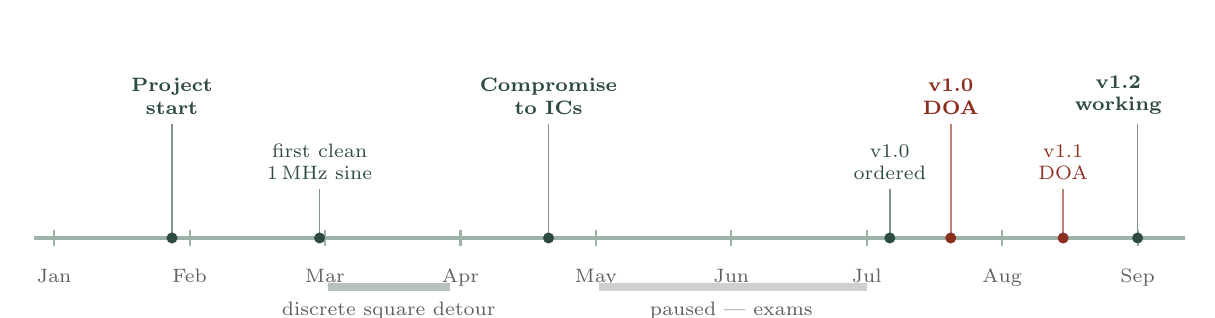
\begin{tikzpicture}[x=1.72cm,y=1cm]
        % baseline
        \draw[line width=1.1pt,accentline] (-0.15,0) -- (8.35,0);
        \foreach \m/\lab in {0/Jan,1/Feb,2/Mar,3/Apr,4/May,5/Jun,6/Jul,7/Aug,8/Sep}{
                \draw[accentline,line width=0.8pt] (\m,-0.1) -- (\m,0.1);
                \node[below=5pt,font=\scriptsize,text=muted] at (\m,-0.1) {\lab};
            }

        % upper tier
        \foreach \x/\txt/\col in {%
        0.87/{Project start}/accent,
        3.65/{Compromise to ICs}/accent,
        6.62/{v1.0 dead on arrival}/fail,
        8.00/{v1.2 working}/accent}{
        \draw[\col!60,line width=0.6pt] (\x,0) -- (\x,1.45);
        \fill[\col] (\x,0) circle (2pt);
        }
        \node[anchor=south,font=\scriptsize\bfseries,text=accent,align=center] at (0.87,1.45) {Project\\start};
        \node[anchor=south,font=\scriptsize\bfseries,text=accent,align=center] at (3.65,1.45) {Compromise\\to ICs};
        \node[anchor=south,font=\scriptsize\bfseries,text=fail,align=center] at (6.62,1.45) {v1.0\\DOA};
        \node[anchor=south east,font=\scriptsize\bfseries,text=accent,align=center] at (8.25,1.45) {v1.2\\working};

        % lower tier
        \foreach \x/\col in {1.96/accent, 6.17/accent, 7.45/fail}{
                \draw[\col!60,line width=0.6pt] (\x,0) -- (\x,0.62);
                \fill[\col] (\x,0) circle (2pt);
            }
        \node[anchor=south,font=\scriptsize,text=accent,align=center] at (1.96,0.62) {first clean\\1\,MHz sine};
        \node[anchor=south,font=\scriptsize,text=accent,align=center] at (6.17,0.62) {v1.0\\ordered};
        \node[anchor=south,font=\scriptsize,text=fail,align=center] at (7.45,0.62) {v1.1\\DOA};

        % spans below
        \draw[line width=3pt,accent!35] (2.02,-0.62) -- (2.92,-0.62);
        \node[below=1pt,font=\scriptsize,text=muted] at (2.47,-0.66) {discrete square detour};
        \draw[line width=3pt,muted!30] (4.02,-0.62) -- (6.0,-0.62);
        \node[below=1pt,font=\scriptsize,text=muted] at (5.0,-0.66) {paused --- exams};
    \end{tikzpicture}
    \caption{Eight months, January to September 2026. Two of the three PCB revisions
        arrived dead; the gap between them is exam season, not debugging.}
    \label{fig:timeline}
\end{figure}

% ================================================================ timeline
\section{Timeline}
\label{sec:timeline}

\subsection{Breadboard era: R-2R, filtering, and a lot of noise}
\label{sec:breadboard}

The project started from nothing on 27 January 2026: Pico toolchain installed, Zadig
drivers for USB, and a first, crude R-2R ladder built from 10\,k\ohm/20\,k\ohm resistors,
driven by AI-generated test firmware for speed. Quality visibly degraded past
60--70\,kHz and the ladder was usable to about 200\,kHz; pushed hard, the bare Pico GPIO
could toggle at up to $\sim$10\,MHz, which set an early --- and, in hindsight,
over-optimistic --- sense of headroom. \srcfile{EngLog 27-01-26 - 0324.txt}

By 18 February the ladder had been changed to 2.2\,k\ohm/1.1\,k\ohm (two 2.2\,k\ohm in
parallel) for better linearity, and serial frequency control was working end to end after
a rewrite of the host I/O code. 1\,MHz looked reachable, by the log's own hedged wording
(``seems that I can manage''), but nothing had been done to condition or verify that
signal yet: the buffer and filter parts it would take to find out were still on the order
list. \srcfile{EngLog 18-02-26 - 1750.txt}

The next entry is the first real filtering attempt: a TL082 unity buffer straight off the
ladder, followed by two RC low-pass stages (470\,\ohm/220\,pF) and a second buffer.
Usable to 100--200\,kHz; at 1\,MHz the signal showed $\sim$50\% amplitude loss, roughly
1\,V of DC offset, and visible jitter and ghosting. Square-wave firmware was added in
parallel but not yet seriously characterised, pending a better op-amp.
\srcfile{EngLog 19-02-26 2036.txt}

\begin{figure}[H]
    \centering
    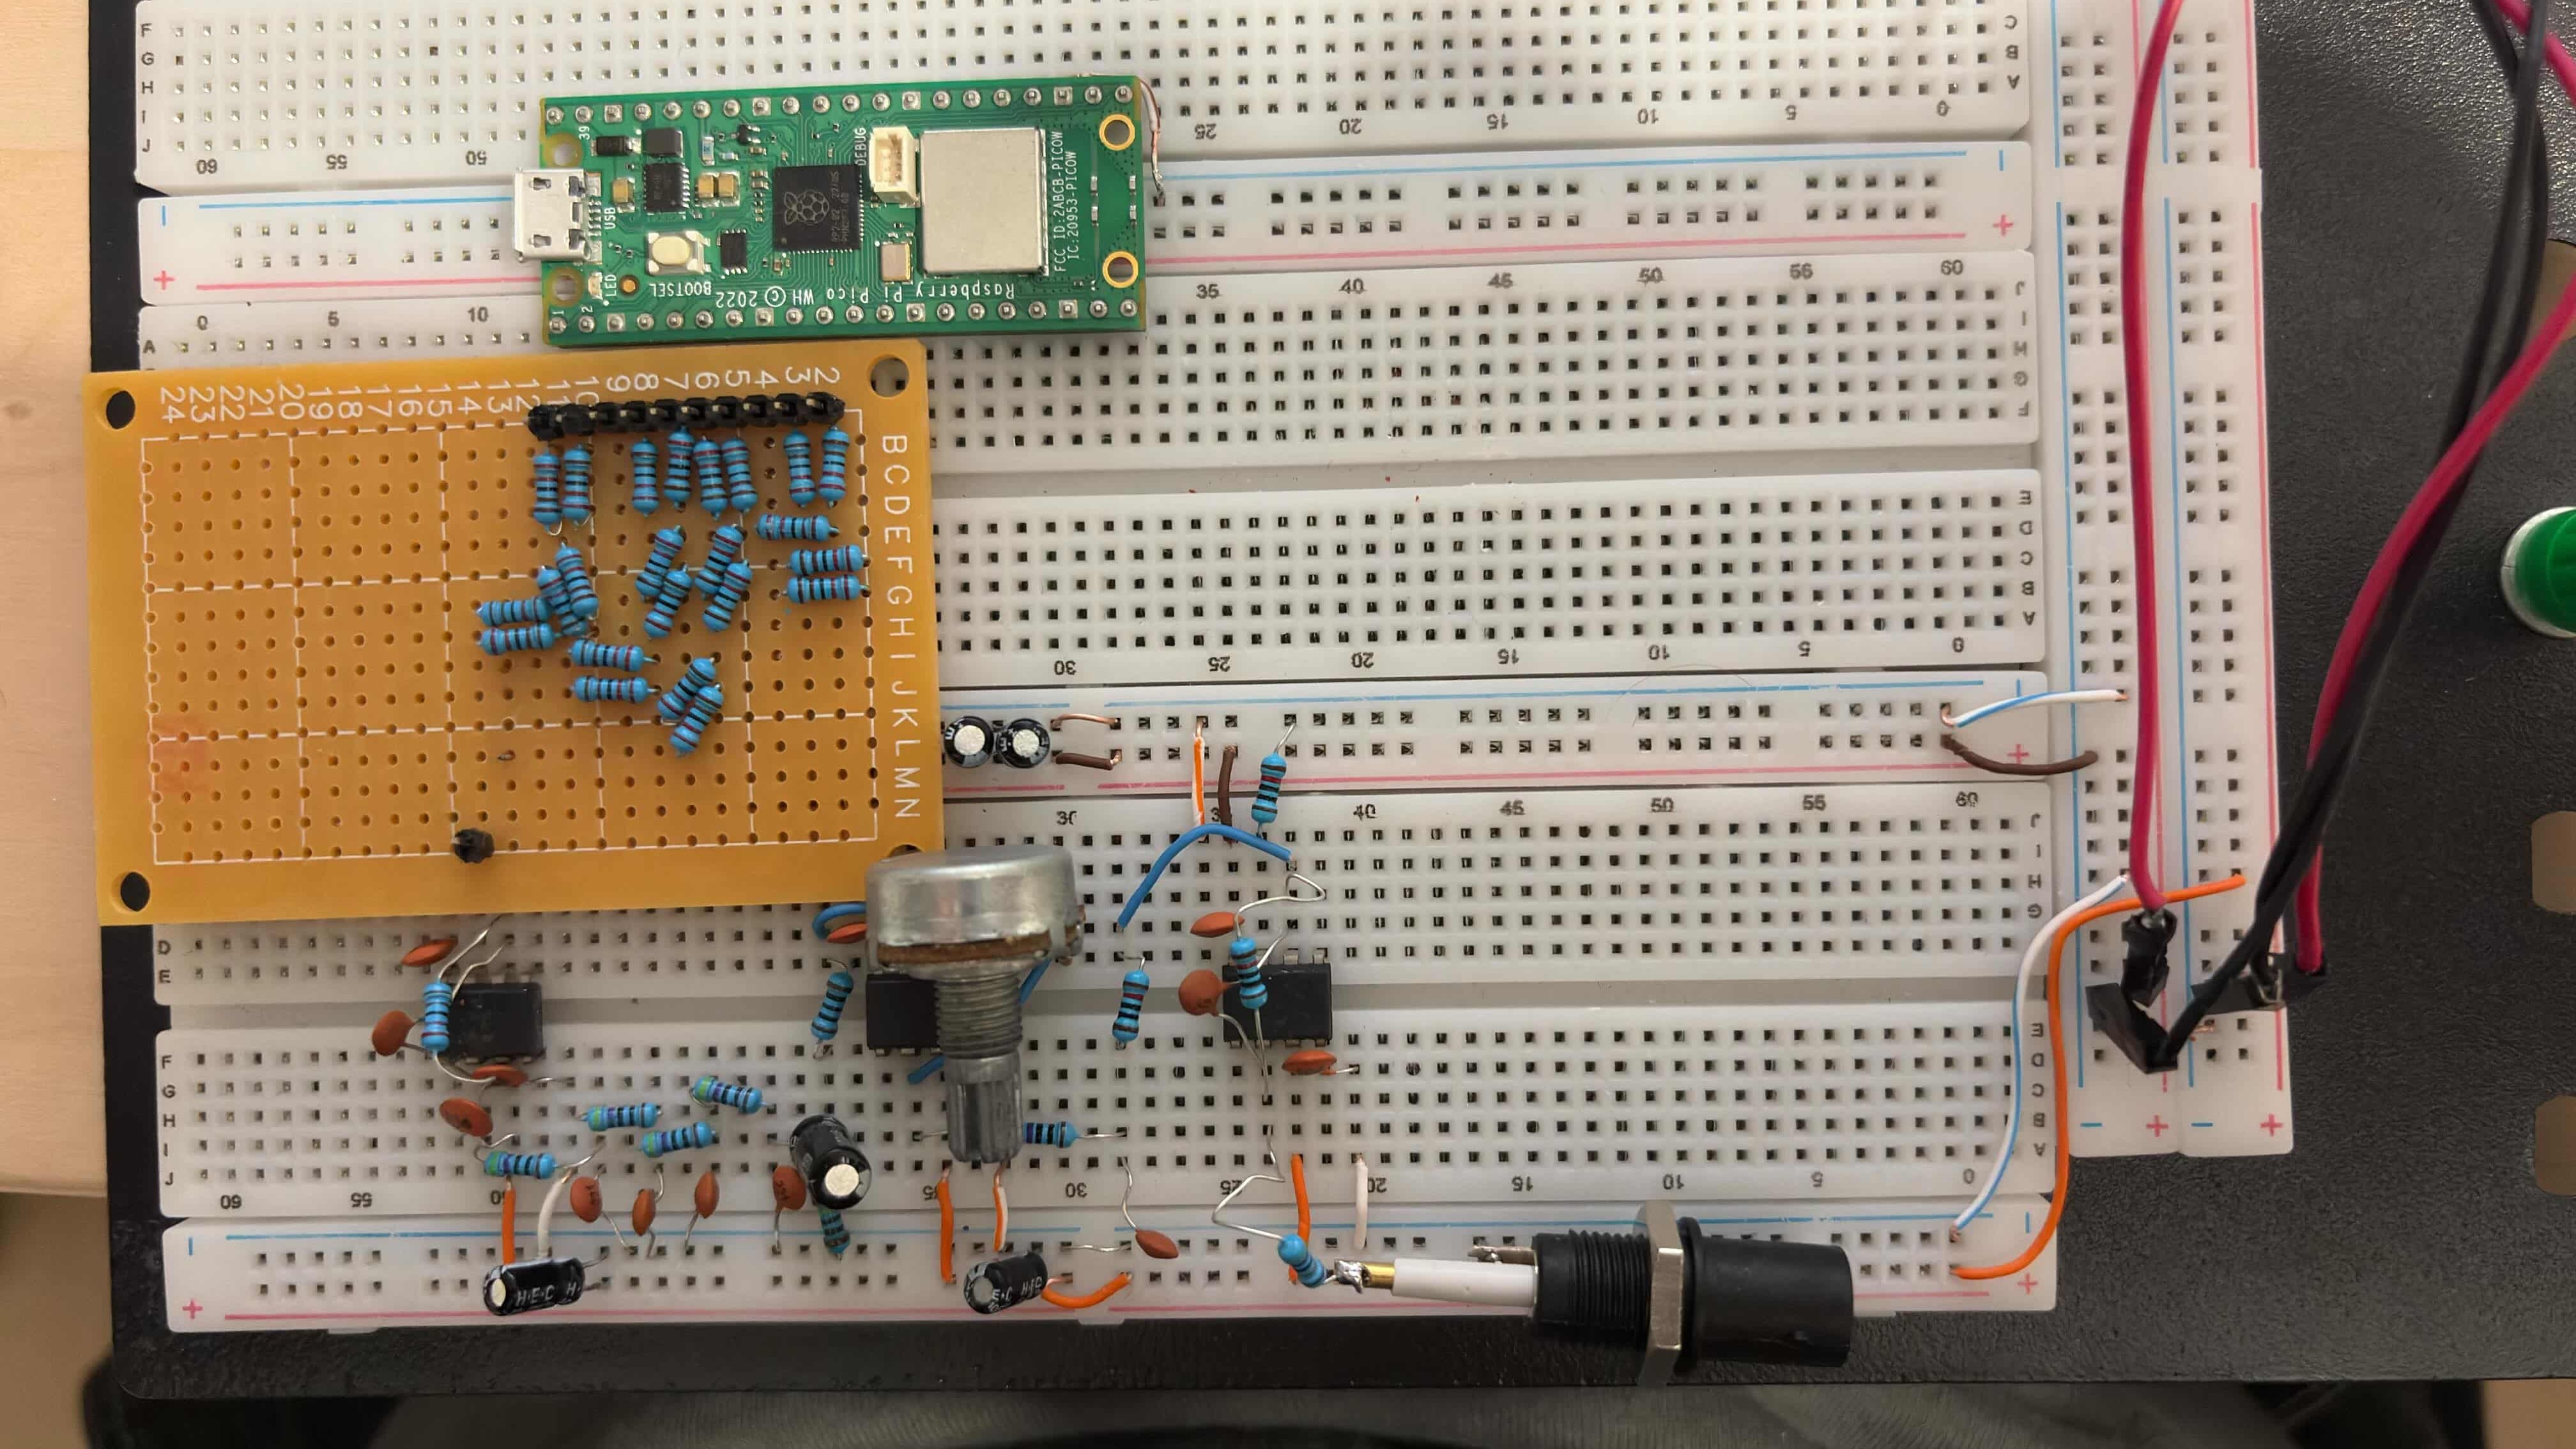
\includegraphics[width=0.62\linewidth]{figures/sinewave_circuit.jpg}
    \caption{Breadboard sine chain during the RC-filter era: R-2R ladder, buffering and
        cascaded filter stages, before the move to LM318 and, later, to a PCB.}
\end{figure}

24 February added a high-pass stage immediately after the ladder to strip the DAC's DC
bias, a 10\,k\ohm potentiometer as a first amplitude control, decoupling
(100\,nF + 10\,\textmu{}F) at the op-amp rails, and the first schematics committed to the
repository. LM318 buffers, solid-core wire and a perfboard were ordered.
\srcfile{EngLog 24-02-26 2100.txt}

\begin{figure}[H]
    \centering
    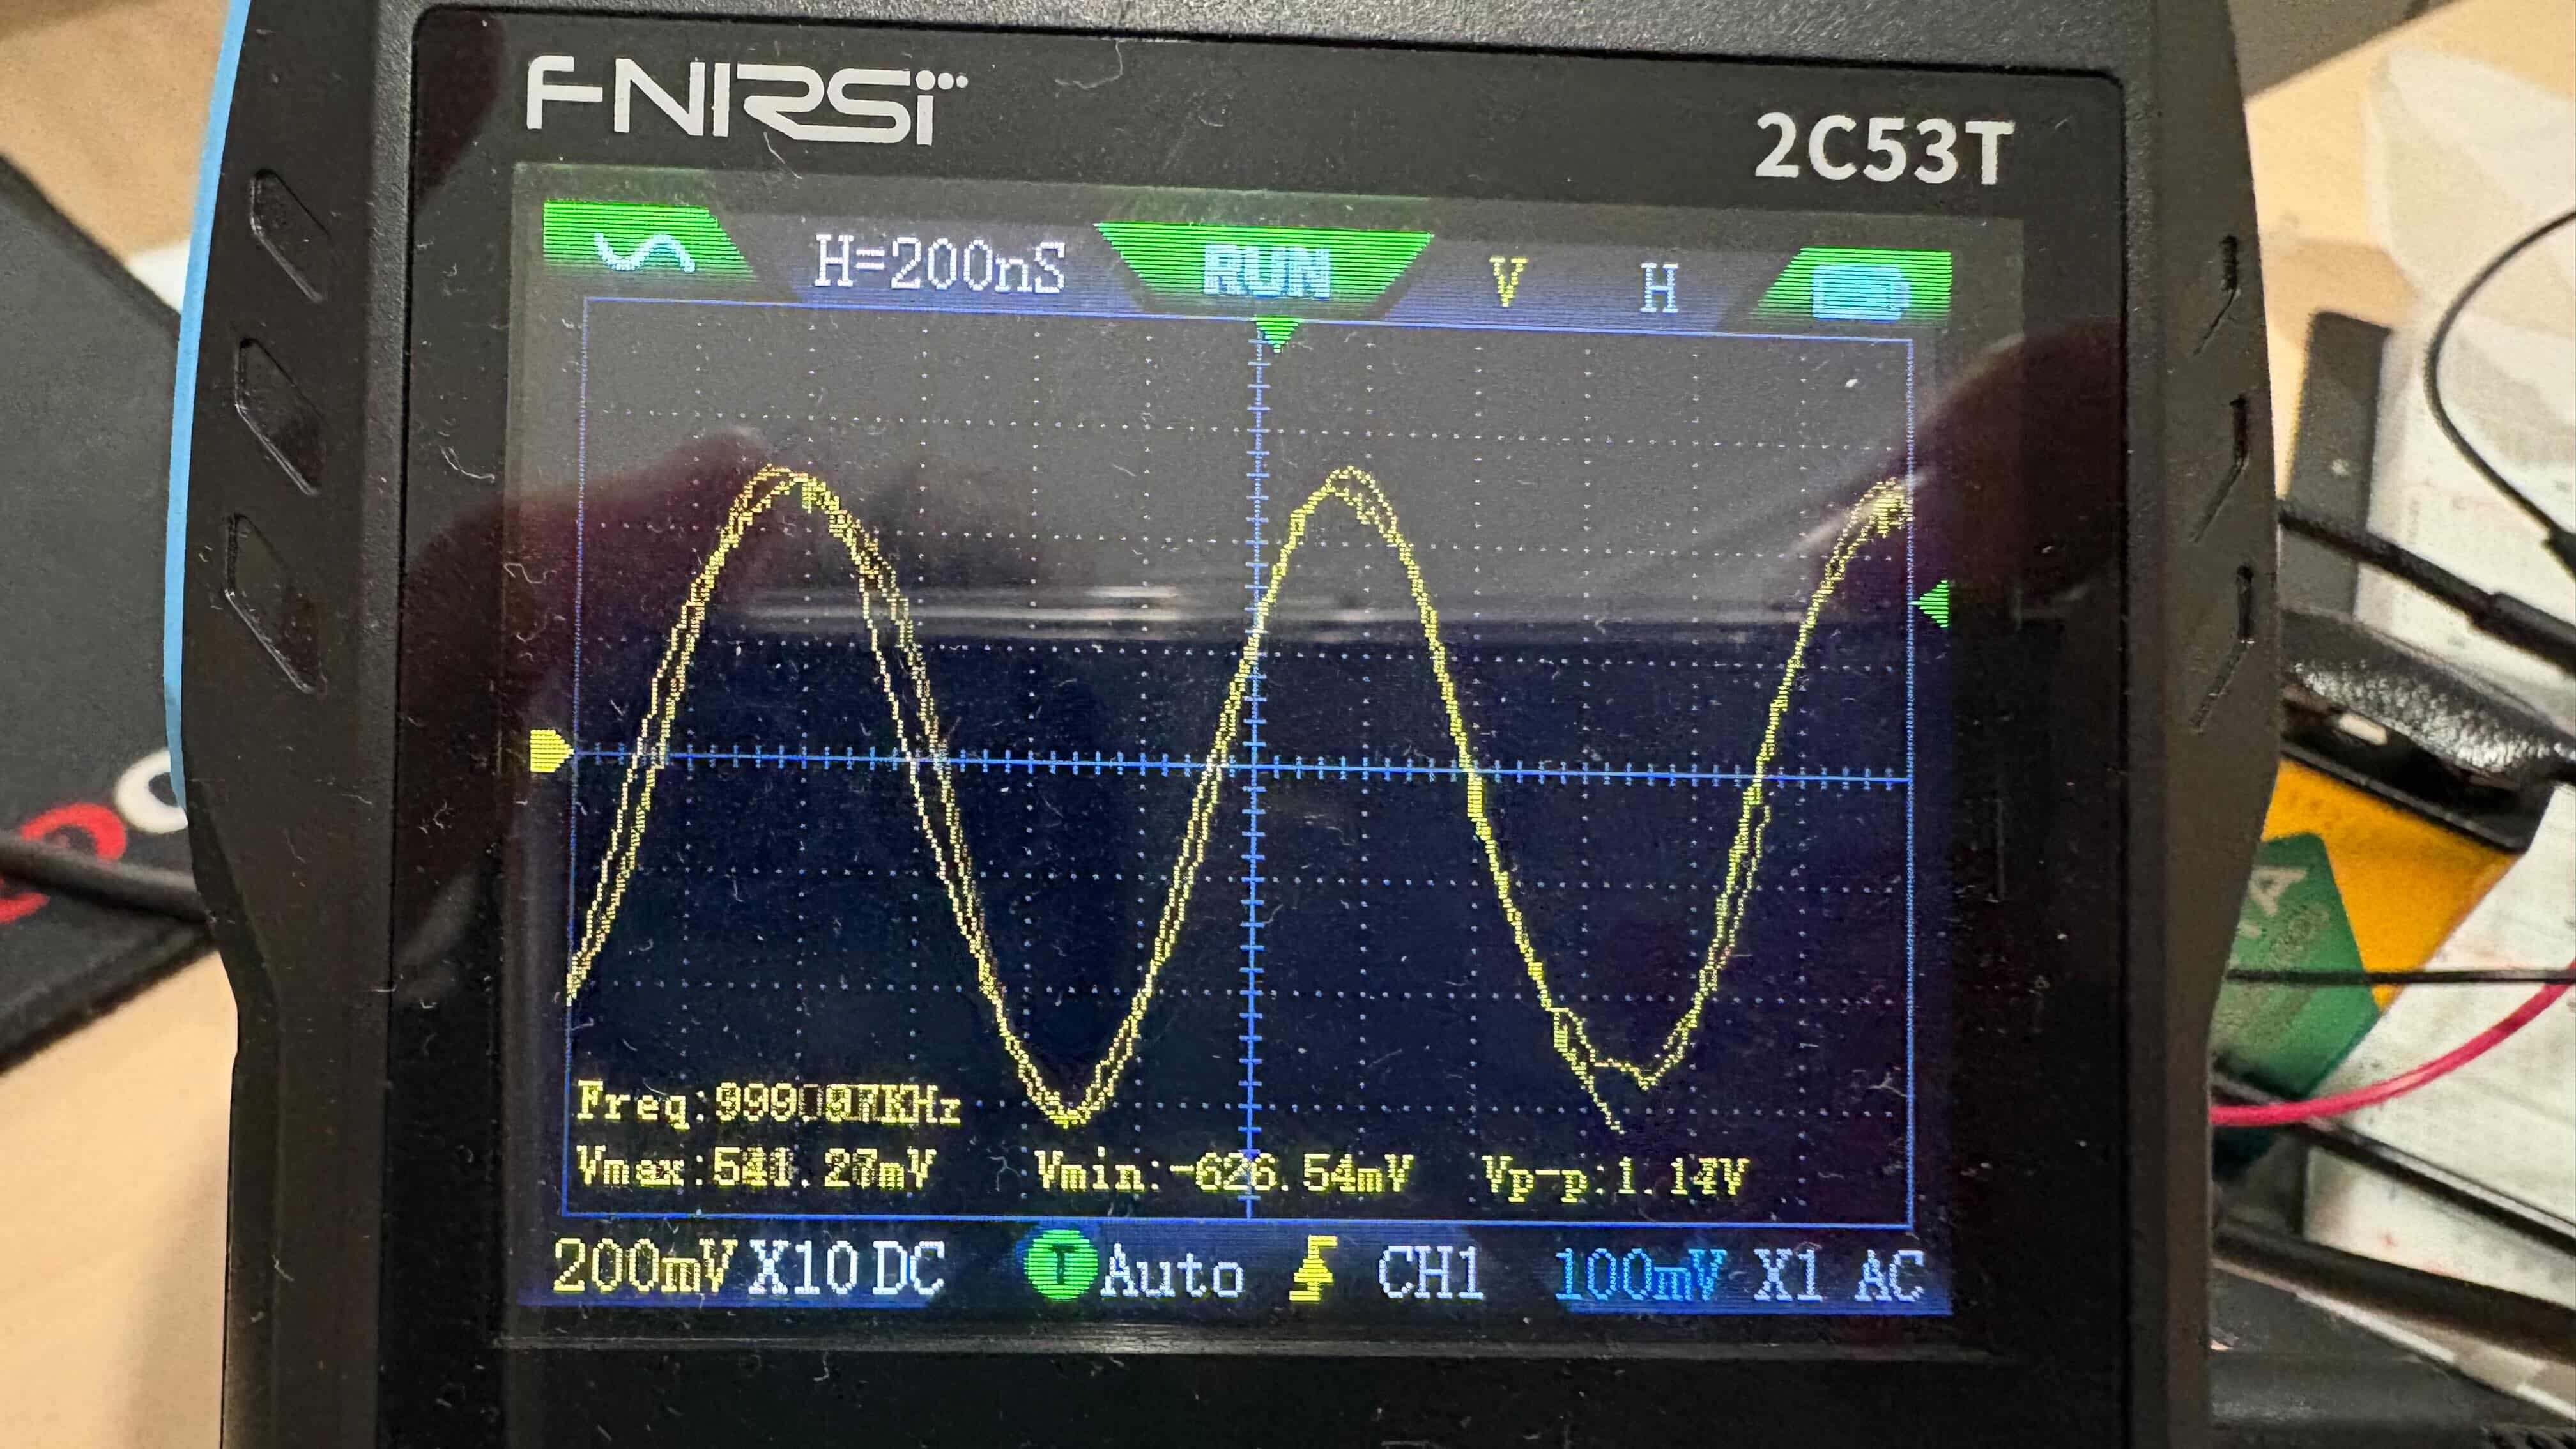
\includegraphics[width=0.62\linewidth]{figures/breadboard_first_quality_check.jpg}
    \caption{First quality check against a bench generator at 1\,MHz, breadboard build.}
\end{figure}

\textbf{The Sallen-Key detour.} With LM318s in hand on 27 February, a full day went into
active Sallen-Key filtering, using parallel resistor and capacitor networks to hit
non-standard ratios. Results were persistently noisy, worse under load, and worse still
through the gain stage. Four candidate causes were ranked in the log itself --- parasitic
capacitance and poor breadboard contact as the top suspect, the unorthodox filter/buffer
layout, bad R-2R contacts newly exposed by the better op-amp, and general wiring and
grounding --- with a closing line that reads, in hindsight, like the project correctly
diagnosing its own next two failure modes:

\begin{quote}
    \itshape ``the brief moments of clean signal with each stage tells me its something
    less\ldots{} systemic.''
\end{quote}
\srcfile{EngLog 27-02-26 0000.txt}

\textbf{First major success.} The very next day, active filtering was abandoned entirely
in favour of five cascaded passive RC stages (four 470\,\ohm/221\,pF low-pass, one
100\,\textmu{}F/1\,M\ohm high-pass), a dedicated inverting gain stage (1\,k\ohm\ input,
0--10\,k\ohm\ feedback pot, 5\,pF compensation) for rail-to-rail swing, a further
low-pass stage to clean up noise the gain stage had uncovered, a voltage-follower output
buffer, and a 47\,\ohm\ series resistor into a BNC connector --- effectively the topology
that would carry through to the PCB. The result was clean, with no ghosting and only a
slight ``vibration'' at 1\,MHz that the log is honest about not being able to attribute to
the circuit rather than the oscilloscope. \srcfile{EngLog 28-02-26 0003.txt}

\begin{figure}[H]
    \centering
    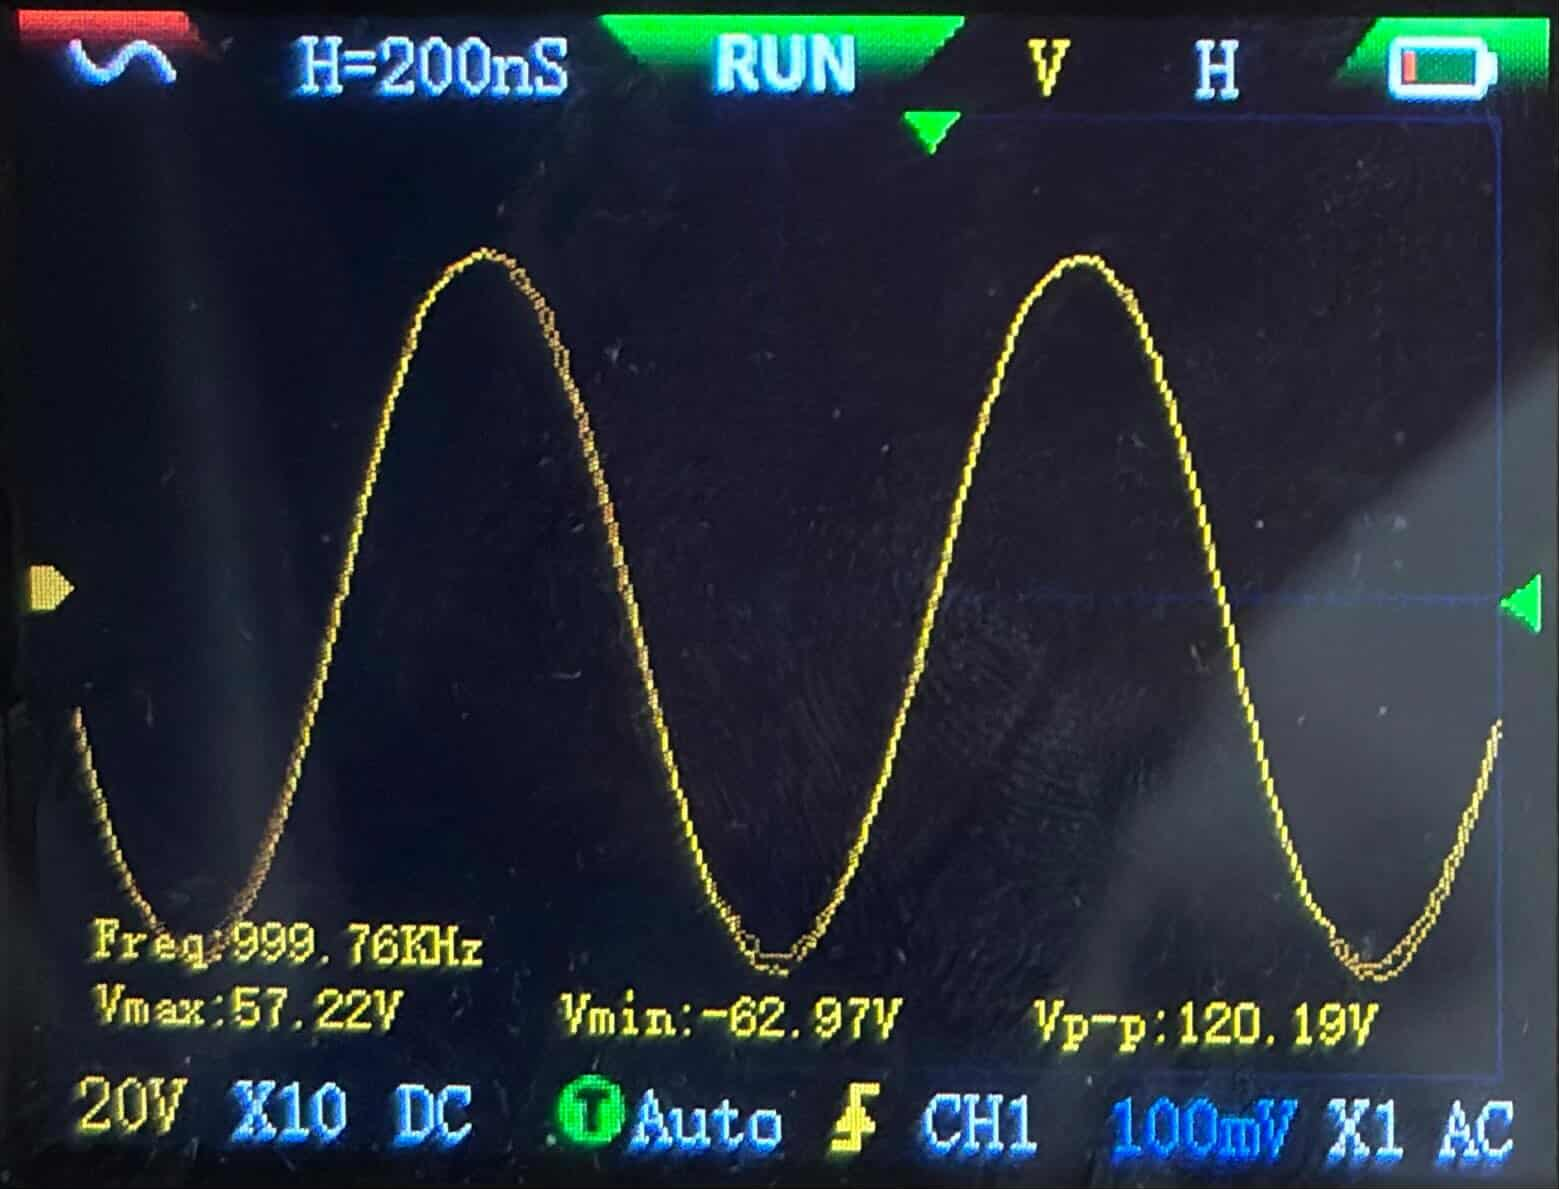
\includegraphics[width=0.62\linewidth]{figures/1MHz_sinewave.jpg}
    \caption{1\,MHz sine capture from the breadboard build, taken around the first
        major success (28 February 2026).}
\end{figure}

\subsection{The discrete square-wave detour}
\label{sec:discrete}

Later the same day, breadboard contact problems fried an LM318 --- a feedback loop opened
under a loose contact. The decision was made to accept the sine chain's Hi-Z-only,
no-current-drive limitations as a deliberate trade for lower parasitics, add square-wave
and arbitrary-waveform output, and move toward a first PCB.
\srcfile{EngLog 28-02-26 1709.txt}

What followed was roughly two weeks of discrete-transistor square-wave buffering, pursued
specifically to build real experience with current amplification rather than reach for an
IC immediately.

\begin{itemize}
    \item \textbf{1 March.} Decision to go discrete; parts ordered.
          \srcfile{EngLog 1-03-26 1637.txt}
    \item \textbf{3 March.} Parts arrive. A hand-derived current amplifier, biased to
          remove the $\sim$0.7\,V junction drop, worked in SPICE but not on the bench. GPIO8 was
          burned by inserting a capacitor believed, incorrectly, to be discharged --- a direct
          hardware casualty rather than a design flaw. \srcfile{EngLog 3-3-26 2336.txt}
    \item \textbf{13 March.} First working square-wave buffer prototype, limited to below
          $\sim$50\,kHz with rounded edges. \srcfile{EngLog 13-03-26 2007.txt}
    \item \textbf{25 March.} An unconventional totem-pole push-pull stage reaches a 1\,MHz
          square wave --- noisy, with a duty-cycle asymmetry the log calls ``duty cycle
          variety'', and limited by a $\sim$1\,k\ohm\ input impedance, visible heating in the
          transistors and resistors, and the battery's own current capacity.
          \srcfile{EngLog 25-03-2026 1739.txt}
    \item \textbf{27 March.} The duty-cycle and frequency-mismatch bugs are traced to the
          first PNP pair's 9\,V rail, and removing it fixes the 1\,MHz case --- but only at high
          frequency; the fix did not carry down to the low-frequency case.
          \srcfile{EngLog 27-03-26 0031.txt}
\end{itemize}

\begin{figure}[H]
    \centering
    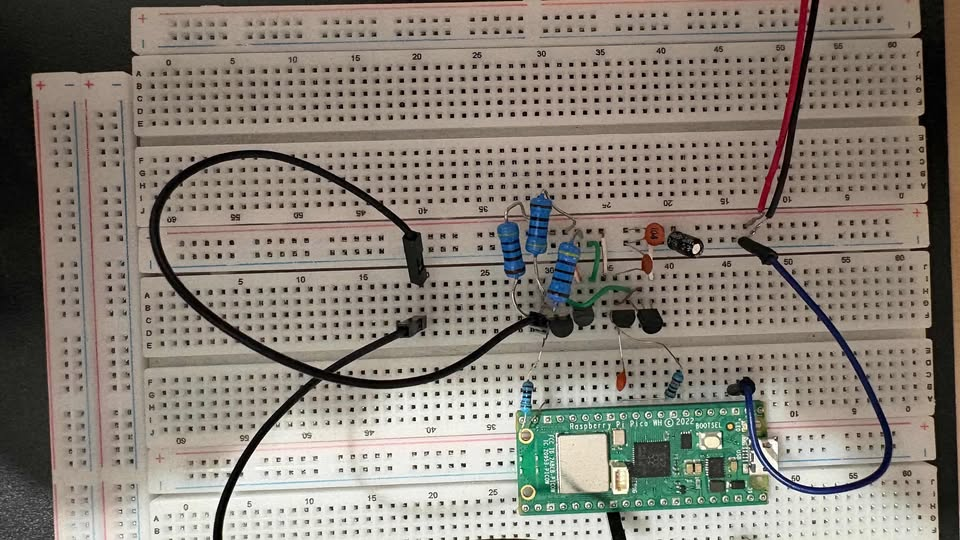
\includegraphics[width=0.5\linewidth]{figures/squarewave.jpg}
    \caption{The discrete-transistor square-wave buffer on breadboard, from this detour
        --- the circuit itself, not a captured output waveform.}
\end{figure}

\subsection{Compromise: ICs, requirements, and a PCB}
\label{sec:compromise}

After the holidays, and after posting for help online without result, the log records a
deliberate compromise: continuing the discrete-transistor path risked never shipping a
working instrument. V1 requirements were fixed --- sine and square from 0 to 1\,MHz at
9\,V peak, digitally adjustable amplitude, PC control via the Pico W, a durable PCB,
strong documentation, BNC output, USB and battery power, and Hi-Z loads only --- and the
square path moved to a TC4427 gate driver, with amplitude control via adjustable LDO rail
limiting (LT3080/LT3090) and a digital pot.

Parts for that scheme were ordered, but neither made it onto the PCB. Simulation showed
the LDO rails degrading the square wave itself, and the digital pot turned out to be
unavailable in the resistance range needed or in a DIP package --- and would have added
noise of its own even if it had been. \srcfile{EngLog 20-04-26 0103.txt}

Project work was then paused through May and into June for exams.
\srcfile{EngLog 01-05-26 1714.txt}

\subsection{v1.0: first PCB, dead on arrival}
\label{sec:v1.0}

The first PCB was designed and ordered as a mixed THT/SMD board --- filtering kept
through-hole for rework access, given how differently breadboard and PCB parasitics were
expected to behave --- using the four-stage cascaded RC filter from the breadboard build.
The rail-limiting amplitude-control scheme from April was tried and dropped: it caused
visible waveform rounding, so amplitude reverted to a simple variable resistor for this
revision. \srcfile{EngLog 6-7-26 1439.txt}

The board arrived, and the failure was immediate and total. The BOM matcher had
substituted 2.21\,\ohm\ resistors for 2.21\,k\ohm\ across the entire R-2R ladder: three
orders of magnitude off, on every rung. This is Lesson~1 in \cref{sec:lessons}.
\srcfile{EngLog 19-07-26 1656.txt}

The same log entry records the immediate pivot: send the board for a respin, replace the
four cascaded RC stages with a 5th-order doubly-terminated LC Butterworth filter
($\sim$1.5\,MHz cutoff, C0G capacitors, 0603 inductors), and move to a fully SMD,
JLCPCB-assembled board. The RC cascade was already a known amplitude bottleneck by this
point --- each stage ate into the signal well before its own corner --- and researching
filter topologies at the time made the Butterworth's flatter passband and steeper rolloff
the obvious replacement, independent of the BOM failure that forced the respin anyway.

\begin{figure}[H]
    \centering
    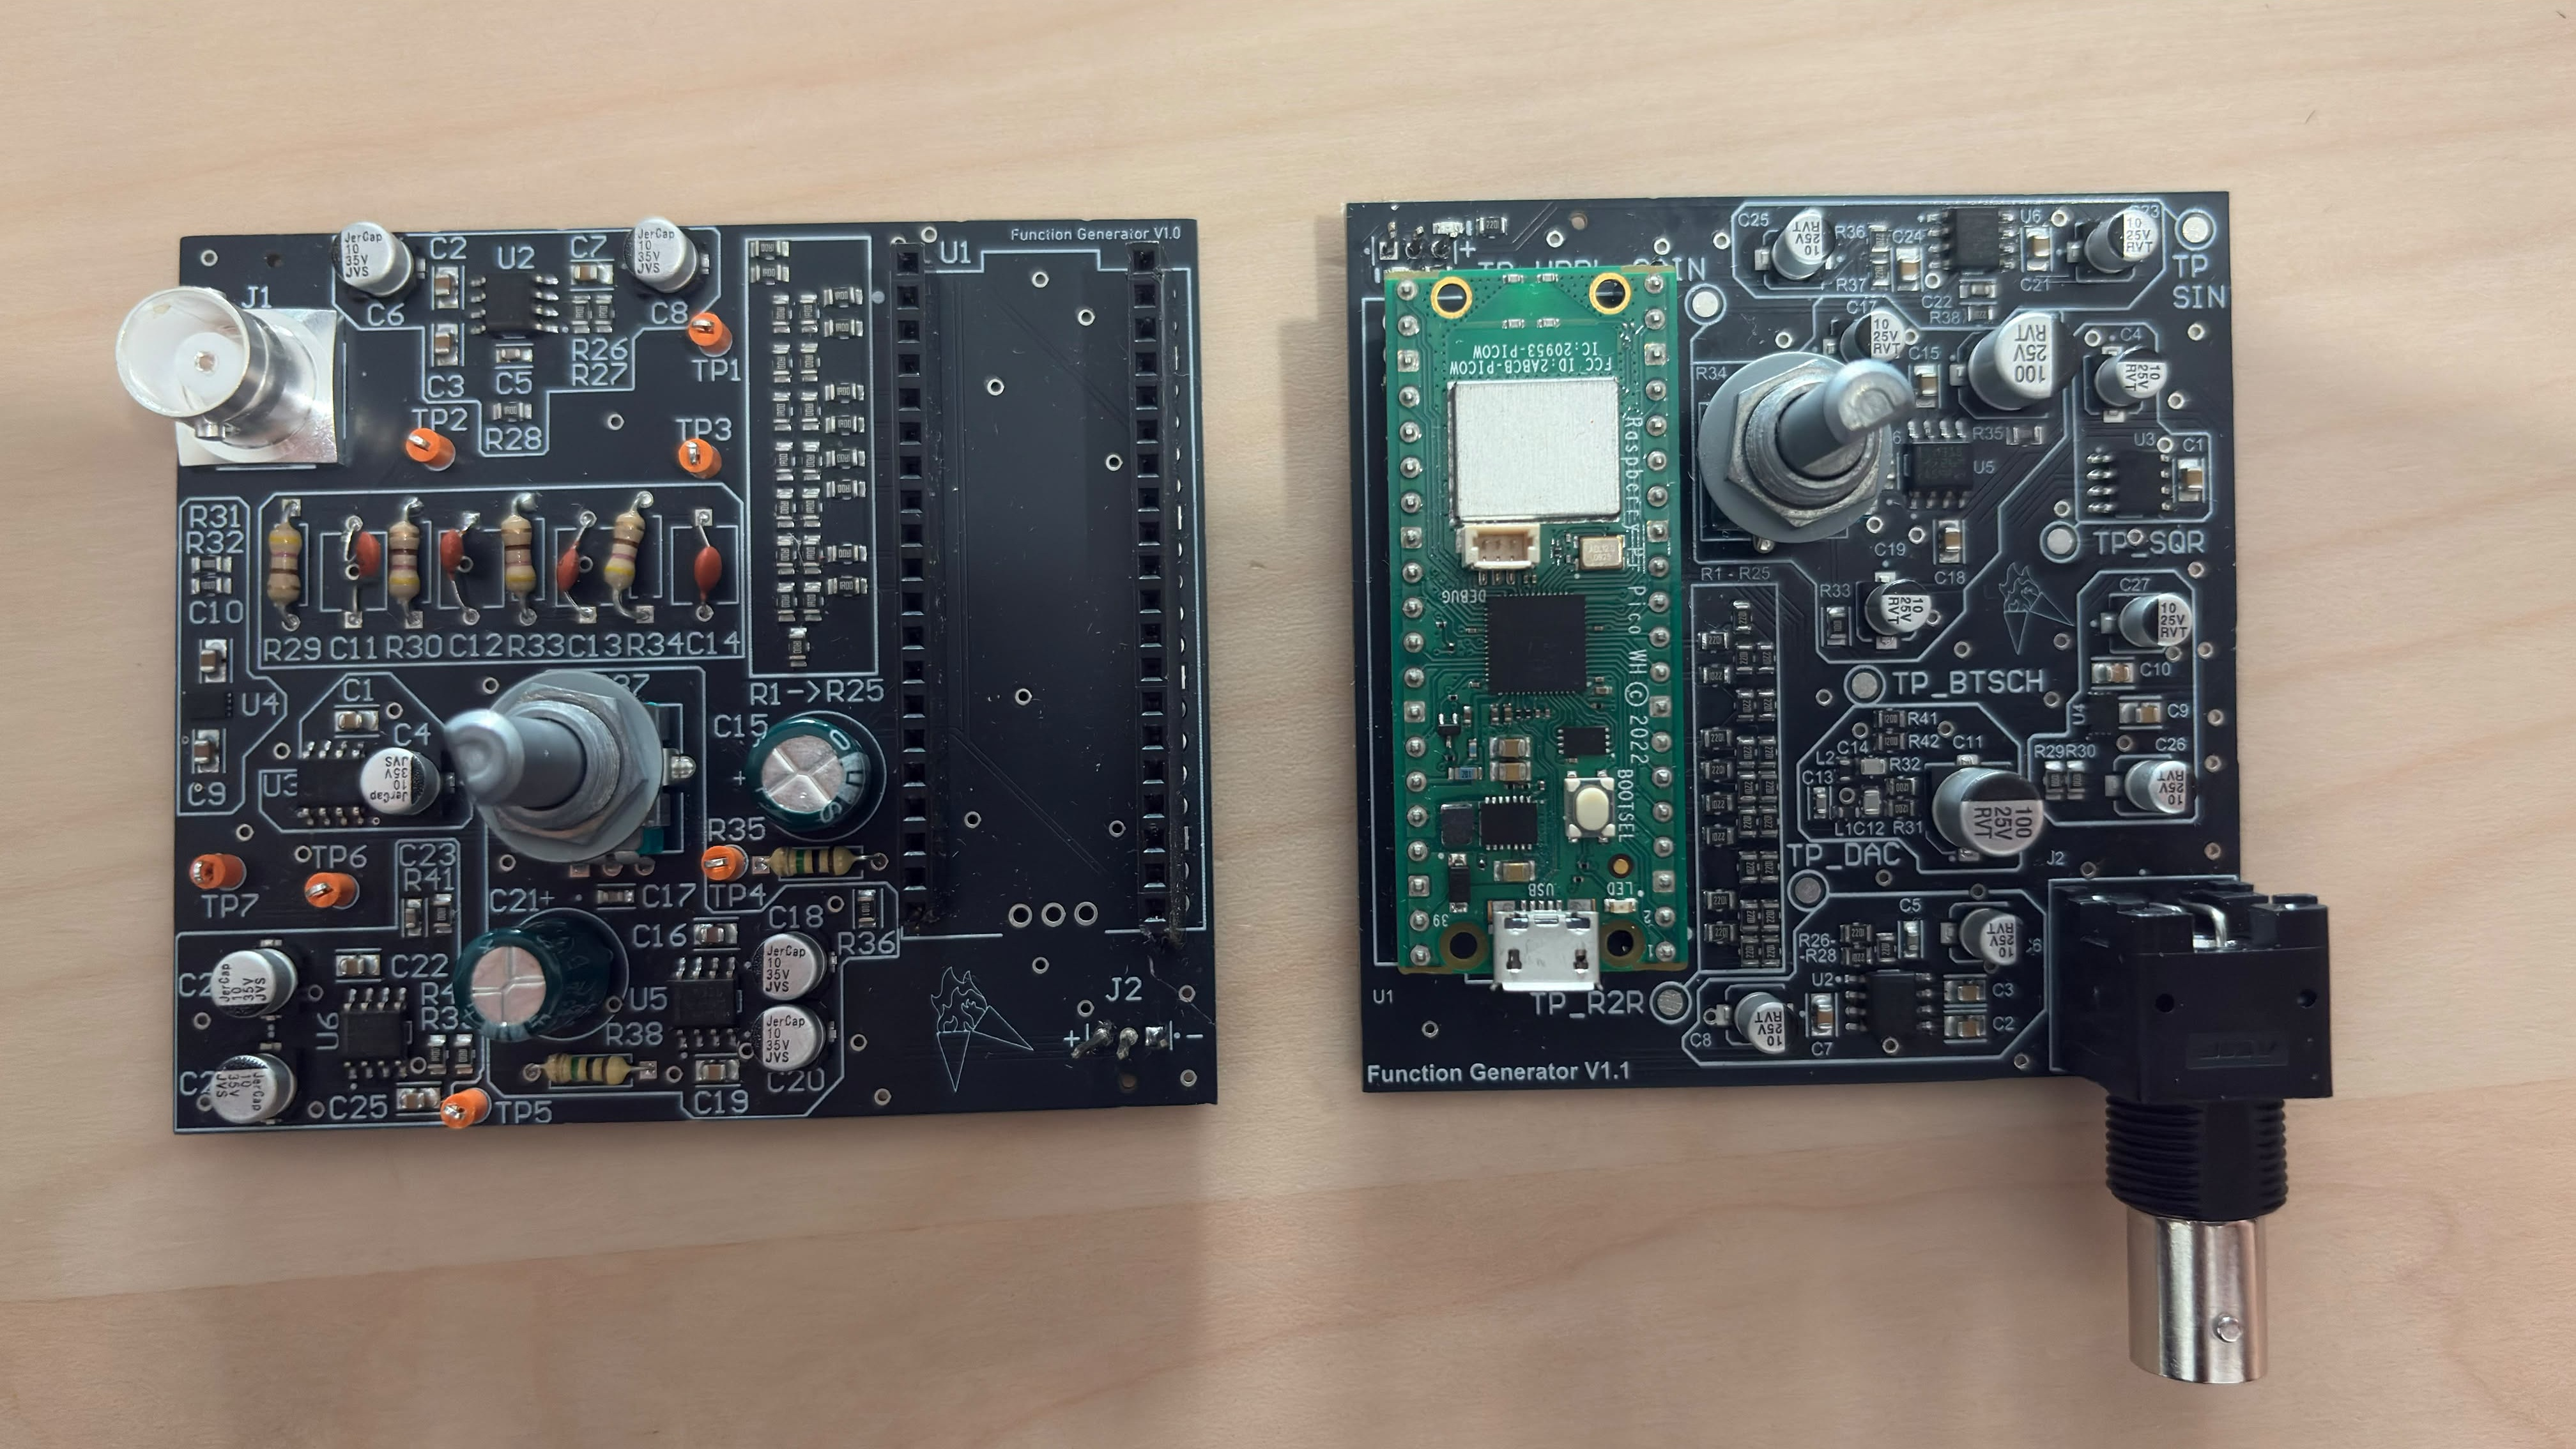
\includegraphics[width=0.82\linewidth]{figures/pcb_v10_v11_dead.jpg}
    \caption{v1.0 (left) and v1.1 (right) side by side --- the two boards that arrived
        dead. v1.0's 2.21\,\ohm\ ladder and cascaded-RC filter section are visible at top
        left; v1.1 already carries the LC Butterworth (L1/L2), the soldered-down Pico and
        the panel-mount BNC that would carry through to v1.2.}
\end{figure}

\subsection{v1.1: Butterworth redesign, dead on arrival}
\label{sec:v1.1}

This version arrived, was soldered up, and went straight to testing --- to no output at
all. The ladder's test point showed nothing and the board was completely silent, with no
immediate way to tell whether the cause was power, firmware or a bad contact.

Pivoting to the square path as a diagnostic step paid off: it worked, and worked well,
with only some edge ringing that turned out to be a probing artefact --- it disappeared
once the scope ground lead was shortened --- rather than a property of the signal. With
sine dead and square clean, the fault was narrowed to the sine chain specifically.

Going over the board repeatedly turned up the cause: a stray trace, left behind during the
KiCad-to-Altium migration, shorting the two inputs of the first-stage LM318. The board's
layout, combined with not having a hot-air rework station on hand, made it impractical to
confirm that this was the \emph{only} fault by reworking and re-testing in place. After
signal insertion at the DAC test point, the rest of the board proved functional at the
lower frequencies the available handheld generator could produce. With the schematic fix
in place, v1.2 was ordered directly.

\begin{caveat}
    No log entry documents this failure or its diagnosis. The account above was supplied
    directly by the author, and \doc{lessons.md}~\#3 is the only other place it is
    summarised.
\end{caveat}

\subsection{v1.2: working build}
\label{sec:v1.2}

With the LM318 short fixed, power LEDs added and costs trimmed in several places, the
board came up clean: tested before assembly, then the Pico soldered directly on. A desktop
host UI was added, along with noise, AM and FM modes on the firmware side. The log calls
the project ``officially completed'' at this point, with bugfixes, additional firmware
features and full characterisation flagged as the next phase rather than as open
requirements. \srcfile{EngLog 01-09026 0306.txt}

\begin{figure}[H]
    \centering
    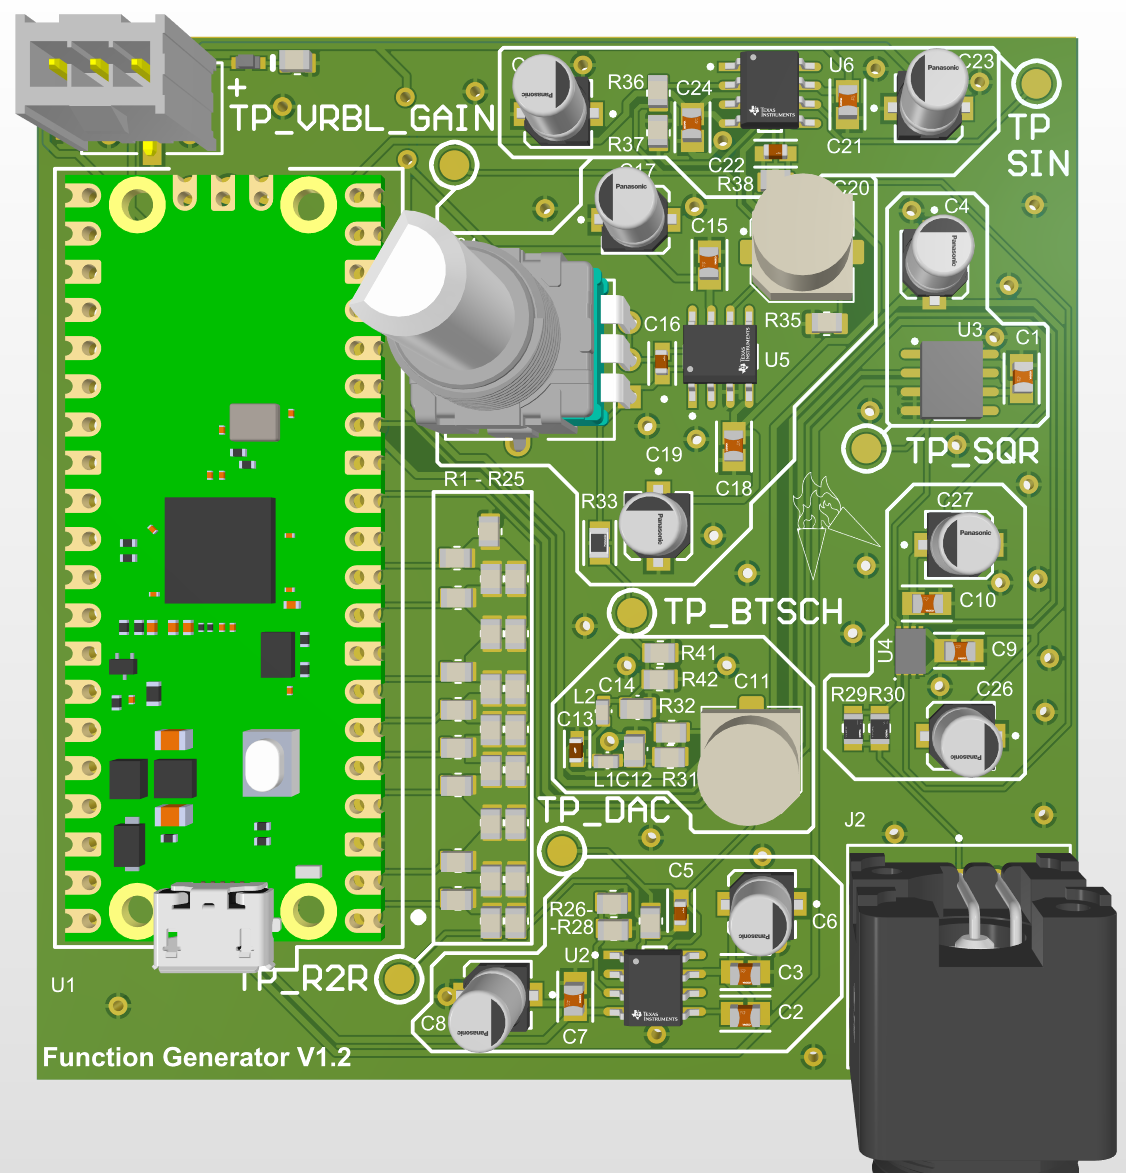
\includegraphics[width=0.48\linewidth]{figures/pcb_3d_render.png}\hfill
    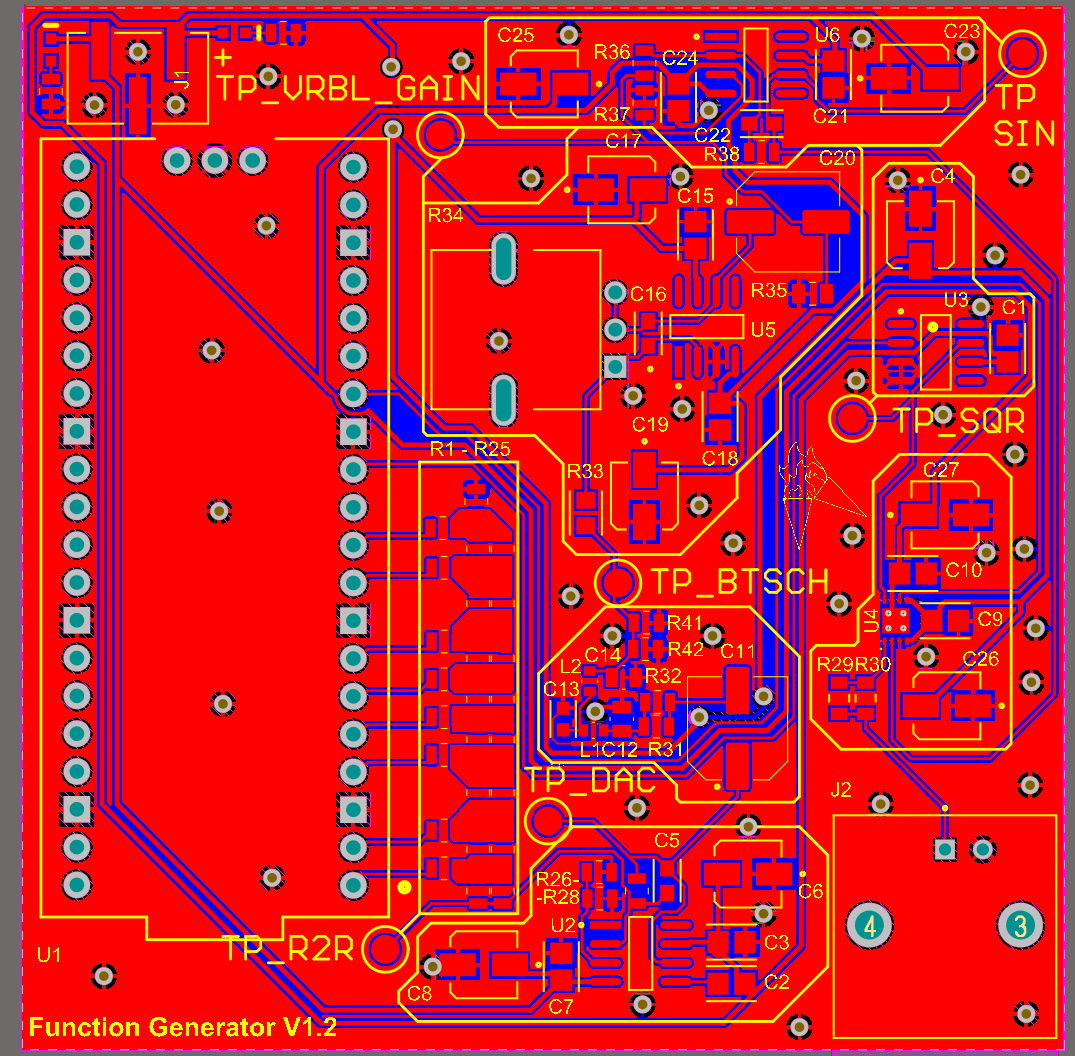
\includegraphics[width=0.48\linewidth]{figures/pcb_layout.png}
    \caption{v1.2 as designed: Altium 3D render and copper layout, August 2026 --- the
        board that was ordered.}
\end{figure}

\begin{figure}[H]
    \centering
    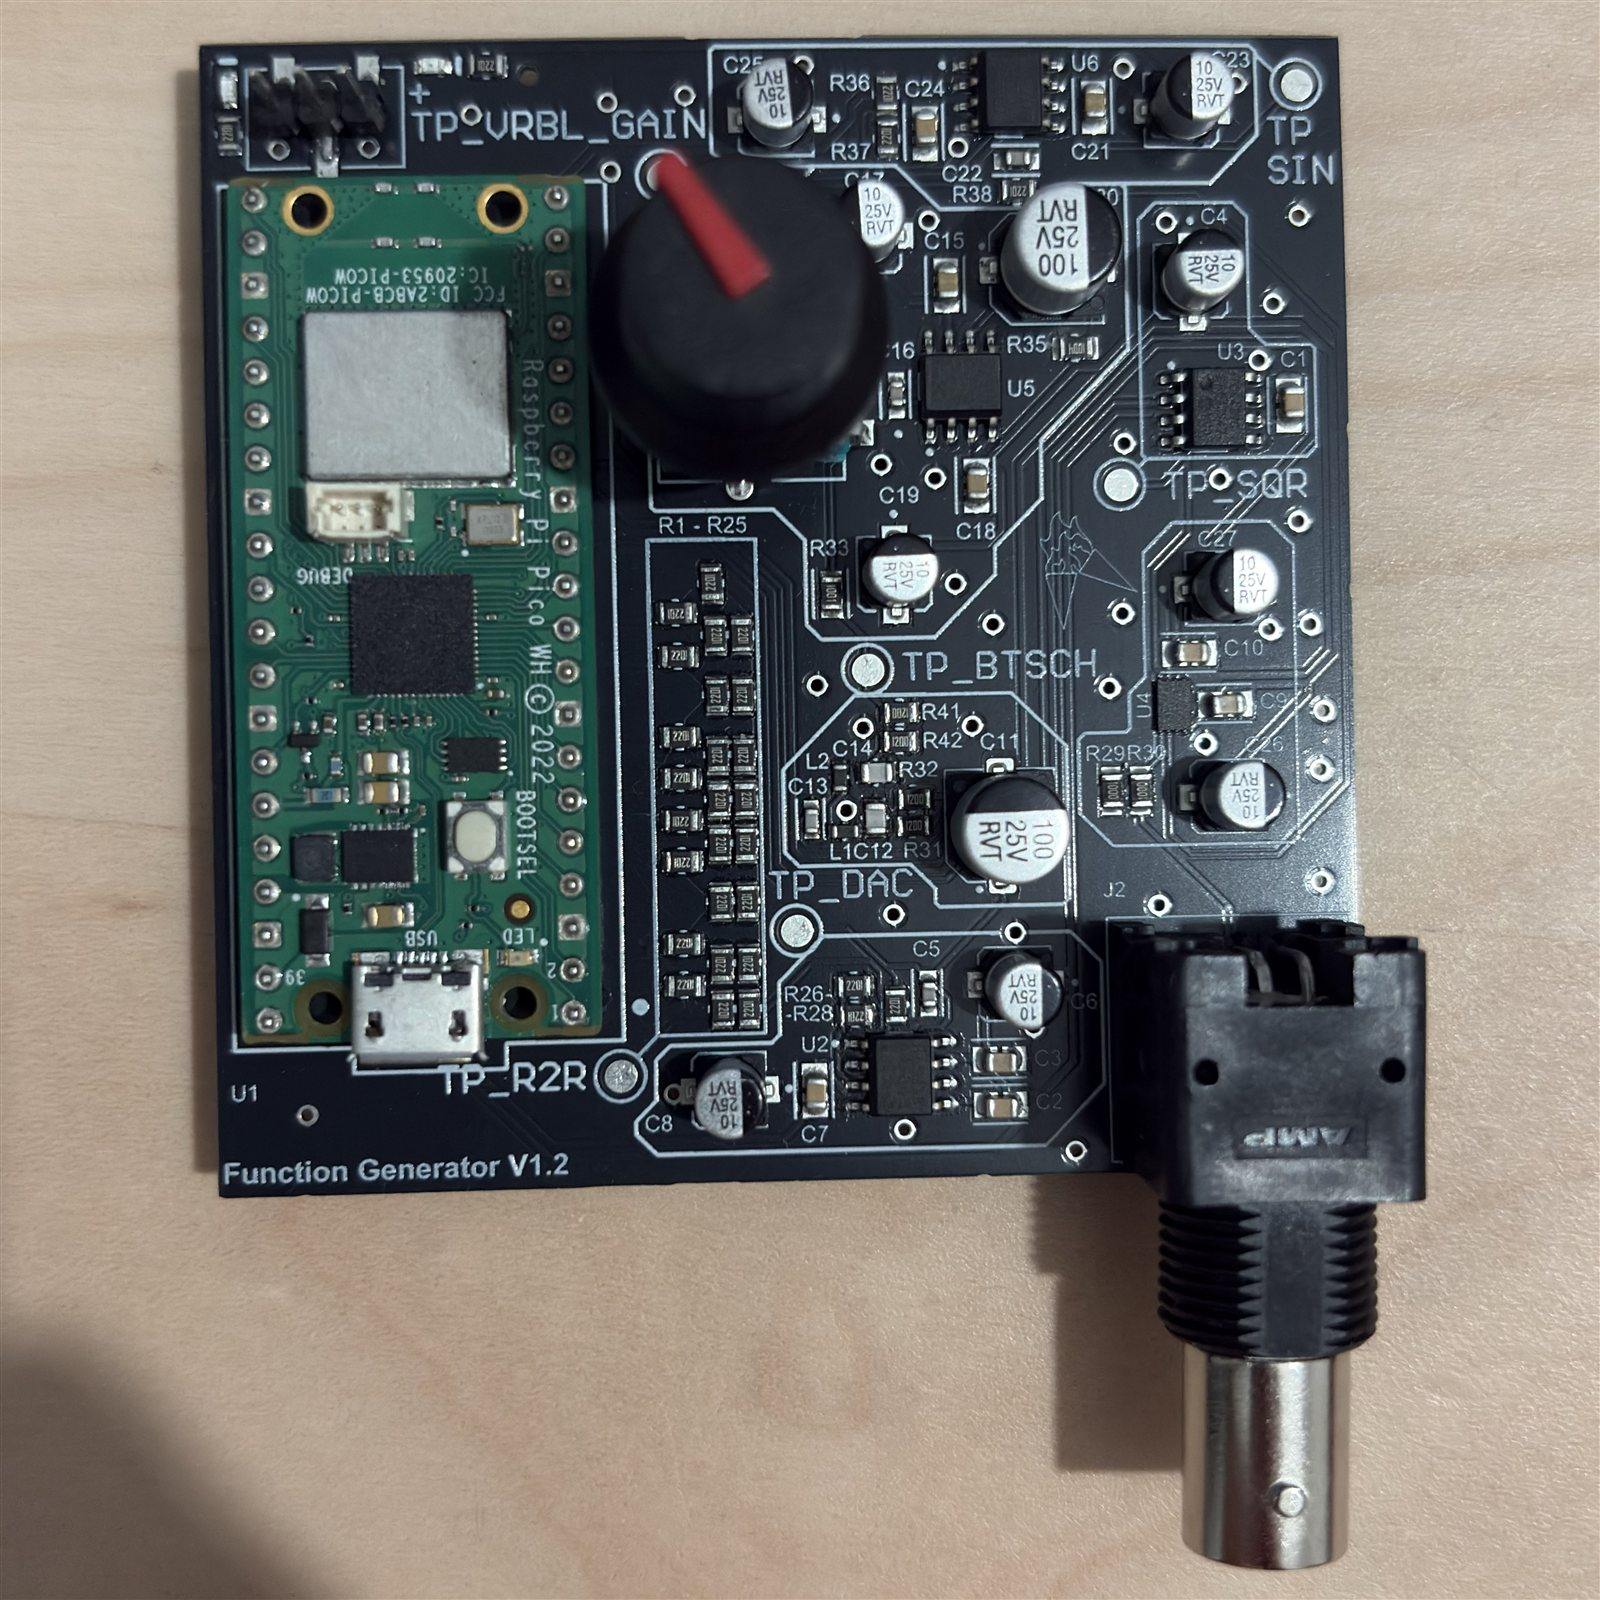
\includegraphics[width=0.62\linewidth]{figures/v12_final_build.jpg}
    \caption{v1.2 as built: the board that arrived, assembled, with the Pico soldered
        directly on and the gain pot and BNC hand-fitted.}
\end{figure}

The very next log entry is where characterisation starts paying off. Full-drive sine
flatness measurements surface a $-3.1$\,dB droop at 1\,MHz, and scaling the DAC lookup
table by four in firmware eliminates it entirely with no hardware change --- which is what
pins the cause on inductor saturation rather than on the filter design or op-amp
bandwidth (Lesson~3, \cref{sec:lessons}). It is diagnosed cleanly and, so far, patched
only in firmware; the real fix is expected to be small, swapping L1/L2 for parts with
adequate saturation current, likely reworkable on the existing board rather than the kind
of fault that forces another respin. A firmware fix for the square wave's duty-cycle
asymmetry is logged in the same entry. \srcfile{EngLog 01-09-2026 1436.txt}

% ================================================================ wrong
\section{What went wrong}
\label{sec:wrong}

\begin{itemize}
    \item \textbf{Every failure that cost a board was invisible to every check that was not
              a physical measurement.} A BOM matcher dropping a unit prefix (Lesson~1), a
          copy-paste merging two nets across an EDA migration (Lesson~2), and a datasheet column
          never read (Lesson~3). None was caught by ERC, DRC, simulation or visual schematic
          review. A fourth, closely related near miss --- name and part-number drift in the
          component library, folded into Lesson~1 alongside the BOM matcher --- was caught early
          enough to cost nothing, which is the only reason it reads as a near miss rather than a
          fourth incident.
    \item \textbf{The Butterworth filter's inductors were selected on inductance, package,
              tolerance and self-resonance --- and not on current rating} (Lesson~3), in a
          60\,\ohm\ system where full-scale drive pushes real current through them. No simulation
          would have surfaced it: LTspice's ideal inductor has no saturation current to violate.
    \item \textbf{Real hardware casualties from real mistakes.} An LM318 fried by a loose
          breadboard contact opening its feedback loop, and GPIO8 burned by inserting a capacitor
          assumed, wrongly, to be discharged (both \cref{sec:discrete}). Both are logged plainly,
          in keeping with this project's own standard for honesty.
    \item \textbf{Two weeks on a discrete square-wave buffer that gave way to an IC anyway.}
          Not a wasted two weeks --- \cref{sec:right} credits the experience --- but the log's own
          tone by late March (``I have realised I grew tired and I'm in way too deep'') is a real
          signal that the discrete-only constraint was fought past the point of being useful, and
          should have been reconsidered sooner.
    \item \textbf{A public request for feedback that produced nothing usable}, noted once
          and not revisited --- worth knowing before trying that channel the same way again.
    \item \textbf{No hot-air rework station on hand when v1.1's LM318 short was found}
          (\cref{sec:v1.1}). With the fault physically identified, the board's layout and the lack
          of that one tool made it impractical to confirm it was the \emph{only} fault by
          reworking in place, so a full respin was ordered on a diagnosis that could not be closed
          out on the bench first.
\end{itemize}

% ================================================================ right
\section{What went right}
\label{sec:right}

\begin{itemize}
    \item \textbf{Killing active filtering when it wasn't working, rather than debugging it
              further.} The Sallen-Key detour (\cref{sec:breadboard}) cost real time, but the decision
          to drop it for passive RC, and later passive LC, rather than chase parasitics in an
          already-suspect breadboard layout, is what produced clean signal the very next day.
    \item \textbf{Diagnosing by changing one variable, twice, at the points that mattered
              most.} The 1\,MHz sine droop was pinned on inductor saturation by scaling the DAC table
          alone and watching the droop disappear with no hardware change (\cref{sec:v1.2}); the
          discrete square buffer's duty and frequency bug was pinned on the first PNP pair's rail by
          removing exactly that (\cref{sec:discrete}). Both are textbook single-variable changes,
          and both are why the causes in this report are stated with confidence rather than hedged.
    \item \textbf{Choosing a passive LC Butterworth over stacking more active stages} once
          the RC cascade's amplitude loss became the limiting factor --- no added op-amp bandwidth
          limit, no added noise, and a much steeper rolloff for the same board complexity.
    \item \textbf{The compromise to use ICs for square-wave buffering.} Two weeks of
          discrete-transistor work (\cref{sec:discrete}) built real understanding of current
          amplification, but the explicit decision to stop and use a TC4427 once shipping was at
          risk is why the project has a working square path at all.
    \item \textbf{Pivoting to the square path as a diagnostic move on v1.1} rather than
          continuing to poke at a completely silent sine chain. A working square output with no
          sine output narrowed the fault to one half of the board immediately, and is what made the
          stray shorted trace findable by review at all (\cref{sec:v1.1}).
    \item \textbf{Soldering the Pico directly to v1.2}, trading reflash convenience --- now
          USB-only --- for the durability a socket does not give a board meant to survive being
          used rather than demonstrated once.
    \item \textbf{Treating ``it compiles clean'' as insufficient evidence.} Both PCB failures
          passed every non-physical check available at the time; the rules derived from them
          (\cref{sec:lessons}) are specifically about closing that gap on the next board, not about
          avoiding the tools that let the errors through.
\end{itemize}

% ================================================================ lessons
\section{Lessons and rules derived}
\label{sec:lessons}

Reproduced from \doc{lessons.md}, which remains the canonical source --- update it there
first if anything here goes stale.

\begin{enumerate}[label=\textbf{\arabic*.},leftmargin=2.1em]
    \item \textbf{BOM and part-identity errors.} Two incidents, same failure class: a part
          gets ordered as something other than what the library says it is, and nothing
          downstream of the library catches it.

          \emph{The 2.21\,\ohm\ incident.} The BOM matcher substituted 2.21\,\ohm\ for
          2.21\,k\ohm\ across the entire R-2R ladder. Cost: one full PCB respin (v1.0).

          \emph{Name and number drift.} Separately, a library entry named as a 0.1\%
          thin-film part carried the LCSC number of a 1\% thick-film part. Harmless in that
          position; the same drift in a precision position would have silently broken the
          design. Caught before it cost anything, which is the only reason it reads as a
          near miss rather than a second respin.
          \begin{itemize}[topsep=0.4em,itemsep=0.35em]
              \item Read the matched part \emph{description} of every BOM line before paying ---
                    value and unit.
              \item Part numbers live at the library level, not per order. The library prevents the
                    error class; the review-page read catches the rest.
              \item Library name, description and LCSC number must agree with each other.
              \item Audit periodically via a parameter-grid view --- inconsistencies are visible in
                    a column that are invisible one component at a time.
              \item Copy the final chosen number back into the library the same day as any
                    order-time substitution.
          \end{itemize}

    \item \textbf{Migration errors.} A KiCad-to-Altium migration merged two LM318 inputs
          onto a single net via a copy-paste that left no visible trace. ERC passed. Cost: one
          full PCB respin (v1.1).
          \begin{itemize}[topsep=0.4em,itemsep=0.35em]
              \item After any cross-EDA paste or import, run ERC \emph{and} a cold continuity check
                    between the input pins of every op-amp instance --- not just the one being worked on.
              \item A schematic that compiles clean is not a schematic that is correct.
          \end{itemize}

    \item \textbf{Maximum current rating.} Butterworth filter inductors were selected on
          inductance, package, tolerance and self-resonance --- not on current rating. Rated
          3\,mA; actual peak current at full scale is $\sim$15\,mA. The saturating ferrite costs
          $-3.1$\,dB at 1\,MHz where the design predicts a flat response.
          \begin{itemize}[topsep=0.4em,itemsep=0.35em]
              \item For series elements in a low-impedance signal path, compute the actual current
                    and check it against the rated and saturation current before selecting --- explicitly,
                    because a 60\,\ohm\ system turns volts into real milliamps in a way that is easy not to
                    think about when reasoning in volts and hertz.
              \item Simulation will not catch this: LTspice inductors are ideal and
                    current-independent.
              \item Hotfix: the firmware low-current mode (lookup table $\div4$) restores linearity
                    at the cost of amplitude and two bits of resolution --- diagnostic-grade, not a fix.
              \item Real fix: the same inductance in a larger package with adequate saturation
                    current.
          \end{itemize}
\end{enumerate}

% ================================================================ current
\section{Current state --- v1.2}
\label{sec:current}

Full numbers live in \doc{measurements.md} and at the top of \repofile{README.md}; this
section is the short version, current as of this report.

\textbf{Working.} Sine from 0\,Hz to 1\,MHz, DDS with a phase accumulator. Square to at
least 2\,MHz, PIO-generated, with user-settable duty and a TC4427-asymmetry correction.
Sine+noise (SNR 0--60\,dB, nominal), AM (0--100\% depth) and FM (deviation in Hz). USB CDC
serial control with a plain-text command protocol and a desktop UI. No DC offset observed.
Output impedance measured rather than assumed: 53\,\ohm\ sine, 58\,\ohm\ square.

\textbf{Known limitations.} Full detail and causes are in \doc{limitations.md}. In short:
the filter inductors are under-rated for the current they actually carry (Lesson~3, with a
firmware workaround rather than a fix); the filter corner sits at $\sim$1.0\,MHz against a
1.5\,MHz simulation and this is still unexplained; the 9\,V-peak output requirement is not
met on $\pm$9.5\,V rails; the instrument drives Hi-Z loads only, with no output buffer
after the switch; amplitude control is an analog pot rather than digital; and THD and
jitter are uncharacterised for lack of equipment.

% ================================================================ open
\section{Open items and future work}
\label{sec:open}

Drawn from \docu{version_requirements.md}{version\_requirements.md} and
\doc{future-work.md}.

\begin{itemize}
    \item \textbf{Digital amplitude control} --- firmware lookup-table scaling, possibly with
          coarse analog gain switching. High priority in \doc{future-work.md}.
    \item \textbf{Noise, AM and FM are implemented and running} but still listed as a future
          requirement, and their key parameters (noise-mode SNR, AM depth) are calculated rather
          than bench-calibrated. Both should be resolved together rather than documented as two
          separate gaps.
    \item \textbf{The DDS paths accept commanded frequencies well past their
              $\sim$2.017\,MHz Nyquist limit with no check}, and alias silently rather than clamp or
          error. This is exactly the mechanism behind the earlier ``2\,MHz sine'' reading that
          turned out to be an alias.
    \item \textbf{Square duty and its correction toggle have no control in the host UI} ---
          serial-only for now.
    \item \textbf{Output impedance is measured on one unit only}; board-to-board variation is
          untested.
    \item \textbf{Deliberately deferred:} higher-voltage output, selectable output impedance,
          output protection, an onboard display, standalone operation and self-calibration all
          remain in \doc{future-work.md}.
\end{itemize}

% ================================================================ appendix
\clearpage
\section*{Appendix A: source material}
\addcontentsline{toc}{section}{Appendix A: source material}
\label{sec:appendix-sources}

\begin{longtable}{@{}ll@{}}
    \toprule
    \rowcolor{accentpale}
    \textbf{\color{accent}Log file}      & \textbf{\color{accent}Covers}                \\
    \midrule
    \endfirsthead
    \toprule
    \rowcolor{accentpale}
    \textbf{\color{accent}Log file}      & \textbf{\color{accent}Covers}                \\
    \midrule
    \endhead
    \texttt{EngLog 27-01-26 - 0324.txt}  & Project start; first R-2R ladder             \\
    \texttt{EngLog 18-02-26 - 1750.txt}  & Serial I/O working; ladder resistor change   \\
    \texttt{EngLog 19-02-26 2036.txt}    & TL082 buffer and filter; square wave added   \\
    \texttt{EngLog 24-02-26 2100.txt}    & HPF, pot, decoupling; schematics started     \\
    \texttt{EngLog 27-02-26 0000.txt}    & Sallen-Key detour; noise-cause ranking       \\
    \texttt{EngLog 28-02-26 0003.txt}    & Passive filter redesign; first major success \\
    \texttt{EngLog 28-02-26 1709.txt}    & LM318 fried; decision to move to PCB         \\
    \texttt{EngLog 1-03-26 1637.txt}     & Decision to go discrete for square wave      \\
    \texttt{EngLog 3-3-26 2336.txt}      & Parts arrive; GPIO8 burned                   \\
    \texttt{EngLog 13-03-26 2007.txt}    & First discrete square buffer ($<$50\,kHz)    \\
    \texttt{EngLog 25-03-2026 1739.txt}  & 1\,MHz totem-pole square prototype           \\
    \texttt{EngLog 27-03-26 0031.txt}    & Duty-cycle and frequency bug fixed           \\
    \texttt{EngLog 20-04-26 0103.txt}    & Compromise to ICs; V1 requirements set       \\
    \texttt{EngLog 01-05-26 1714.txt}    & Project paused for exams                     \\
    \texttt{EngLog 6-7-26 1439.txt}      & v1.0 PCB ordered                             \\
    \texttt{EngLog 19-07-26 1656.txt}    & v1.0 DOA (2.21\,\ohm); v1.1 re-order decided \\
    \emph{(author account, no log file)} & v1.1 DOA; LM318 short found and diagnosed    \\
    \texttt{EngLog 01-09026 0306.txt}    & v1.2 complete; UI, noise, AM, FM added       \\
    \texttt{EngLog 01-09-2026 1436.txt}  & Inductor saturation found; duty cycle fixed  \\
    \bottomrule
\end{longtable}

\begin{caveat}[title={Note on that one row}]
    No log entry documents v1.1's own failure or its diagnosis. That account
    (\cref{sec:v1.1}) was supplied directly by the author, and \doc{lessons.md}~\#3 is the
    only other place it is summarised.
\end{caveat}

% ================================================================ schematic
\clearpage
\section*{Appendix B: current schematic (v1.2)}
\addcontentsline{toc}{section}{Appendix B: current schematic (v1.2)}
Dated 26 August 2026, reproduced at full page width overleaf. The embed is vector ---
scroll or pinch-zoom reads every net and value losslessly --- and the schematic is
also a link: click it to open
\href{https://github.com/Lambros25/Function-Generator/blob/main/hardware/schematic_overview.pdf}{\texttt{hardware/schematic\_overview.pdf}}
on GitHub, a
real URL that works from anywhere this PDF is opened, phone included, unlike a
relative path into a folder that may not travel with the file.

\begin{landscape}
    \begin{figure}[H]
        \centering
        \href{https://github.com/Lambros25/Function-Generator/blob/main/hardware/schematic_overview.pdf}{%
            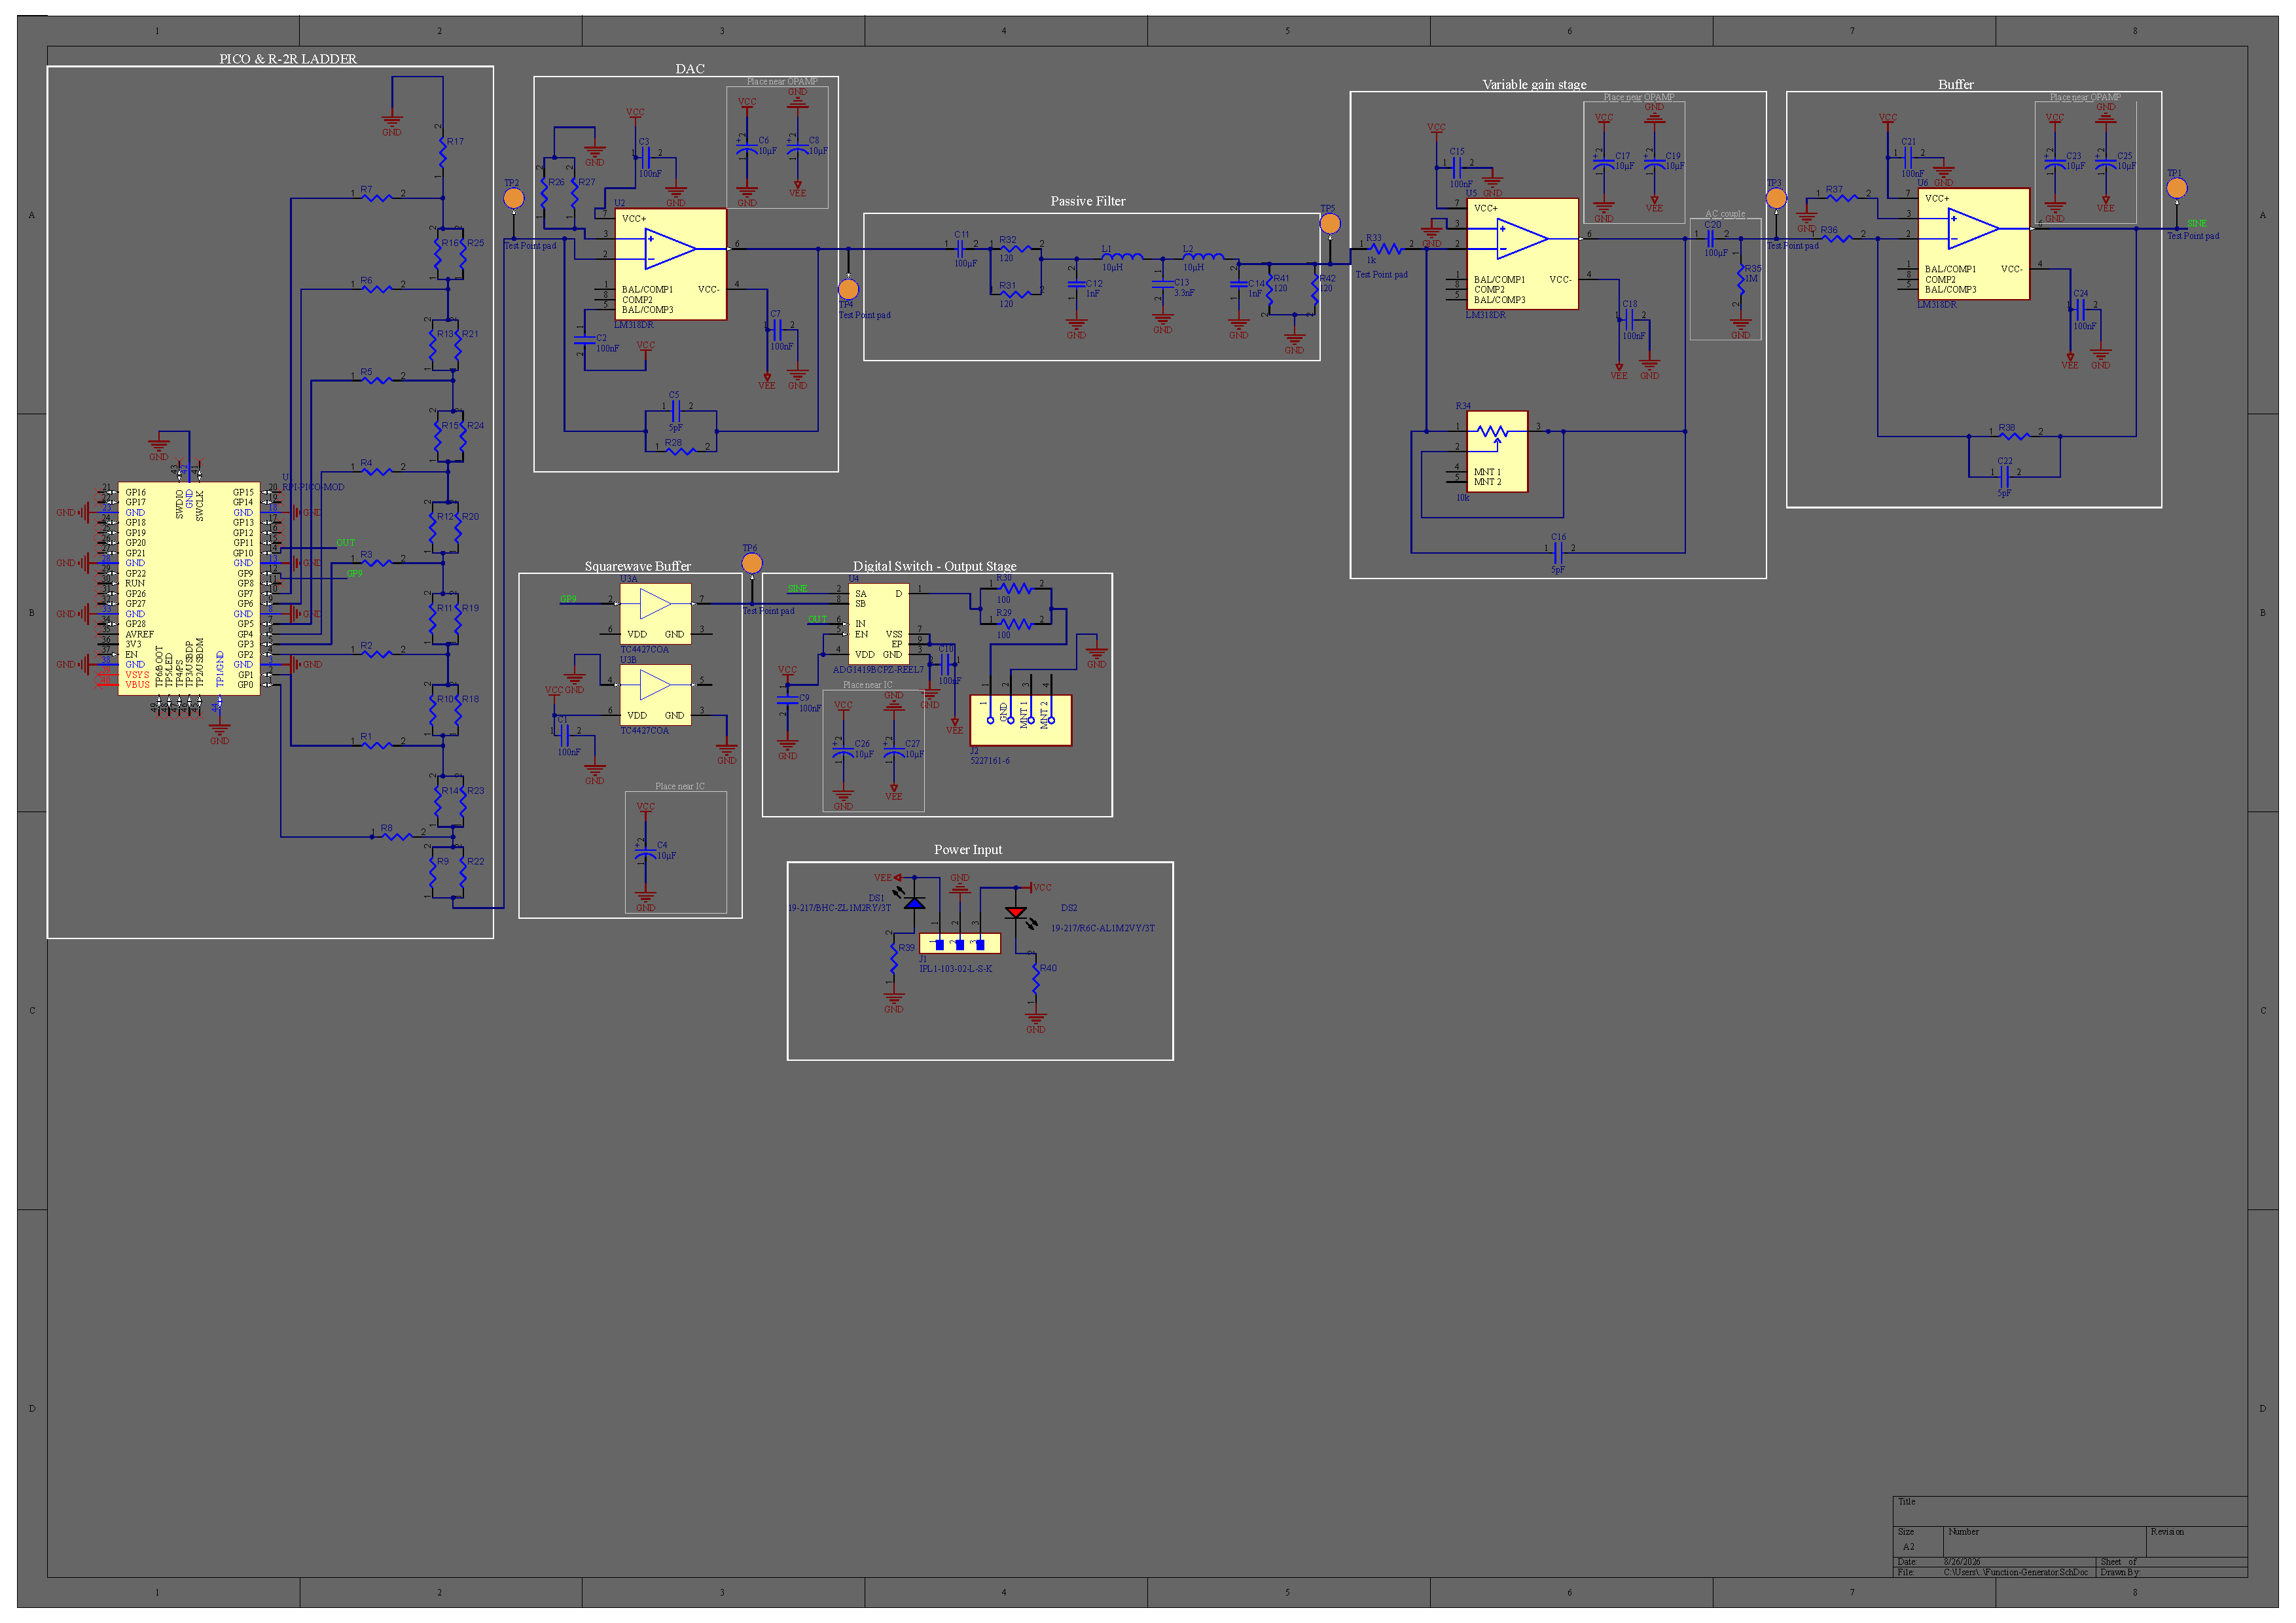
\includegraphics[width=0.85\linewidth]{figures/schematic_overview.pdf}}
    \end{figure}
\end{landscape}

\end{document}